%=====================================================================
%  The University of Danang - Journal of Science and Technology (UD-JST)
%  Laid out to match the official UD-JST Word template:
%    paper 190 x 265 mm, margins 1 cm, Times New Roman 10 pt,
%    two columns, gap 0.5 cm, single line spacing, 3 pt before/after,
%    default tab stop 0.5 cm.
%  All figures and tables are single-column.
%  Compile: xelatex main.tex  (run twice)
%=====================================================================
\documentclass[10pt,twocolumn,twoside]{article}

\usepackage[paperwidth=190mm,paperheight=265mm,
            left=10mm,right=10mm,top=10mm,bottom=15mm,
            headheight=12pt,headsep=6pt,footskip=10mm]{geometry}
\setlength{\columnsep}{5mm}

\usepackage{fontspec}
\setmainfont{TeX Gyre Termes}          % metric-compatible with Times New Roman
\usepackage{polyglossia}
\setmainlanguage{english}
\setotherlanguage{vietnamese}

\usepackage{graphicx}
\usepackage{multirow}
\usepackage{array}
\usepackage[table]{xcolor}
\usepackage{amsmath}
\usepackage{amssymb}
\usepackage{caption}
\usepackage{subcaption}
\usepackage{titlesec}
\usepackage{fancyhdr}
\usepackage[hidelinks]{hyperref}
\usepackage{tikz}
\usetikzlibrary{arrows.meta, positioning, shapes.geometric}

% ---- paragraph and line spacing (template: before 3pt / after 3pt) ---
\setlength{\parindent}{0.5cm}          % default tab stop 0.5 cm
\setlength{\parskip}{3pt}
\linespread{1.0}

% ---- captions:  "Figure 1." bold, caption text italic, centred --------
\captionsetup[figure]{font={small,it},labelfont={small,bf,up},
                      labelsep=period,justification=centering,
                      skip=3pt,position=bottom}
\captionsetup[table]{font={small,it},labelfont={small,bf,up},
                     labelsep=period,justification=centering,
                     skip=3pt,position=top}

% ---- headings (template style) ---------------------------------------
% 1.<tab>Heading 1      : bold
% 1.1.<tab>Heading 2    : bold italic
% 1.1.1.<tab>Heading 3  : italic
\titleformat{\section}{\bfseries\normalsize}{\thesection.}{0.5cm}{}
\titleformat{\subsection}{\bfseries\itshape\normalsize}{\thesubsection.}{0.4cm}{}
\titleformat{\subsubsection}{\itshape\normalsize}{\thesubsubsection.}{0.4cm}{}
\titlespacing*{\section}{0pt}{6pt}{3pt}
\titlespacing*{\subsection}{0pt}{5pt}{2pt}
\titlespacing*{\subsubsection}{0pt}{5pt}{2pt}

% ---- running heads: rule kept, no header text; page number centered ---
% ---- in the footer (bottom margin/footskip enlarged above to fit it) --
\pagestyle{fancy}
\fancyhf{}
\fancyfoot[C]{\thepage}
\renewcommand{\headrulewidth}{0.4pt}
\renewcommand{\footrulewidth}{0pt}

% ---- reference list: normal-size numbers in square brackets ----------
\makeatletter
\renewcommand\@biblabel[1]{[#1]}
\makeatother

\begin{document}

% placed after \begin{document}: polyglossia resets \figurename/\tablename
% per-language at \begin{document}, which would otherwise clobber a
% preamble-level \renewcommand for these names
\renewcommand{\figurename}{Hình}
\renewcommand{\tablename}{Bảng}

%=====================================================================
%  TITLE BLOCK  (spans both columns)
%=====================================================================
\newsavebox{\titleblock}
\begin{lrbox}{\titleblock}
\begin{minipage}{\textwidth}
\setlength{\parindent}{0pt}
\begin{center}
{\bfseries\large
Báo cáo tiến độ\par}
\vspace{4pt}
{\large
Ngày \number\day\ tháng \number\month\ năm \number\year\par}
\vspace{8pt}
\end{center}

% Overview diagram is embedded directly in the spanning title block
% (rather than as a floating figure*) so it is guaranteed to render
% immediately below the title, before any section text -- a figure*
% placed after \twocolumn[...] cannot also claim the same page's single
% top-of-page float slot and would otherwise be deferred to page 2.
\centering
\resizebox{0.92\textwidth}{!}{%
\begin{tikzpicture}[
  node distance=9mm and 10mm,
  box/.style={rectangle, rounded corners, draw=black, thick, fill=blue!10,
              align=center, minimum height=9mm, minimum width=30mm, font=\small},
  decision/.style={diamond, draw=black, thick, fill=orange!15, align=center,
                   font=\small, aspect=2.6, inner sep=1pt},
  aggbox/.style={rectangle, rounded corners, draw=black, thick, fill=violet!12,
                 align=center, minimum height=9mm, minimum width=27mm, font=\small},
  outbox/.style={rectangle, rounded corners, draw=black, thick, fill=green!10,
                 align=center, minimum height=9mm, minimum width=30mm, font=\small},
  arrow/.style={-{Latex[length=2.2mm]}, thick}
]

\node[box, fill=gray!15] (input) {Phổ NIR đầu vào\\$\mathbf{x} \in \mathbb{R}^{D}$};

\node[box, above right=9mm and 18mm of input] (clf) {SMART-NIR\\(Phân loại)};
\node[aggbox, right=10mm of clf] (aggclf) {K-Fold ($K{=}5$)\\Bỏ phiếu};
\node[outbox, right=10mm of aggclf] (catout) {Loại thực phẩm\\(9 lớp)};

\node[box, below right=9mm and 18mm of input] (stage1) {XGBoost\\(Bước 1 -- Phát hiện)};
\node[aggbox, right=10mm of stage1] (aggstage1) {K-Fold ($K{=}5$)\\Bỏ phiếu};
\node[decision, right=10mm of aggstage1] (haspesticide) {Có\\thuốc trừ sâu?};
\node[outbox, above right=5mm and 8mm of haspesticide] (negout) {Không phát hiện};
\node[box, below right=5mm and 8mm of haspesticide] (stage2) {SMART-NIR\\(Bước 2 -- Định lượng)};
\node[aggbox, right=10mm of stage2] (aggstage2) {K-Fold ($K{=}5$)\\Trung bình};
\node[outbox, right=10mm of aggstage2] (regout) {Nồng độ thuốc trừ sâu\\(mg/kg)};

\draw[arrow] (input) -| (clf);
\draw[arrow] (clf) -- (aggclf);
\draw[arrow] (aggclf) -- (catout);
\draw[arrow] (input) -| (stage1);
\draw[arrow] (stage1) -- (aggstage1);
\draw[arrow] (aggstage1) -- (haspesticide);
\draw[arrow] (haspesticide) -| node[above,pos=0.3,font=\scriptsize]{Không} (negout);
\draw[arrow] (haspesticide) -| node[below,pos=0.3,font=\scriptsize]{Có} (stage2);
\draw[arrow] (stage2) -- (aggstage2);
\draw[arrow] (aggstage2) -- (regout);

\end{tikzpicture}%
}
\vspace{4pt}
\captionof{figure}{Sơ đồ tổng quan hệ thống, giải quyết đồng thời ba bài
toán: phân loại loại thực phẩm, phát hiện sự hiện diện và dự đoán nồng độ
thuốc trừ sâu. Mỗi mô hình được huấn luyện theo kiểm định chéo K-Fold
(K-Fold cross-validation, $K{=}5$); dự đoán cuối cùng của một mẫu tổng hợp
từ 5 mô hình theo fold bằng bỏ phiếu đa số (majority voting) khi phân
loại/phát hiện, hoặc trung bình cộng khi định lượng.
Nhánh phát hiện/định lượng (Bước 1 -- Bước 2) được lặp lại độc lập cho từng
loại trong 19 thuốc trừ sâu khảo sát.}
\label{fig:overview}
\end{minipage}
\end{lrbox}

\twocolumn[\usebox{\titleblock}\vspace{14pt}]

%=====================================================================
\section{Phương pháp}

\subsection{Tổng quan}

Hệ thống được xây dựng nhằm giải quyết đồng thời ba bài toán từ cùng một phổ
NIR đầu vào của một mẫu rau củ quả: (1) phân loại loại thực phẩm; (2) phát
hiện sự tồn tại của từng loại thuốc bảo vệ thực vật trong mẫu; và (3) dự đoán
hàm lượng (nồng độ) của thuốc bảo vệ thực vật đó nếu được xác định là có tồn
tại. Sơ đồ tổng quan của hệ thống được minh họa trong Hình~\ref{fig:overview}.

Bài toán (1) được giải quyết độc lập bằng một mô hình SMART-NIR
(Mục~\ref{sec:smartnir}) đóng vai trò bộ phân loại đa lớp, với số lớp đầu ra
tương ứng số loại rau củ quả (9 lớp). Mô hình được huấn luyện theo kiểm định
chéo K-Fold ($K=5$, Mục~\ref{sec:clf-training}), tạo ra 5 mô hình độc lập
theo từng fold; ở bước suy luận, dự đoán cuối cùng cho một mẫu được tổng hợp
từ 5 mô hình này bằng bỏ phiếu đa số (majority voting) thay vì chỉ dùng một
mô hình đơn lẻ, giúp giảm phương sai và tăng độ ổn định của kết quả phân
loại.

Bài toán (2) và (3) được giải quyết theo một quy trình lai gồm hai bước, lặp
lại độc lập cho từng loại trong số 19 thuốc trừ sâu khảo sát. Cả hai bước
đều huấn luyện theo kiểm định chéo K-Fold ($K=5$, Mục~\ref{sec:stage-training})
và tổng hợp dự đoán từ 5 mô hình theo fold ở bước suy luận:
\begin{itemize}
\setlength{\itemsep}{1pt}
\item \textbf{Bước 1 -- Phát hiện.} Mô hình XGBoost (Mục~\ref{sec:xgboost})
được sử dụng như một bài toán phân loại nhị phân, xác định thuốc trừ sâu đang xét
có tồn tại trong mẫu hay không; giống bài toán (1), quyết định cuối cùng được
tổng hợp bằng bỏ phiếu đa số (majority voting) qua 5 mô hình theo fold.
\item \textbf{Bước 2 -- Định lượng.} Chỉ những mẫu được Bước 1 xác định là
có tồn tại thuốc trừ sâu mới được đưa tiếp vào Bước 2, tại đó một mô hình
SMART-NIR đóng vai trò bộ hồi quy, huấn luyện riêng cho từng thuốc trừ sâu, được
dùng để dự đoán giá trị nồng độ; do đầu ra là giá trị liên tục, dự đoán cuối
cùng là trung bình cộng của 5 dự đoán theo fold thay vì bỏ phiếu (voting).
\end{itemize}

Cách tiếp cận theo tầng (cascade) này mang lại ba lợi ích: (i) tránh lãng phí
năng lực của mô hình hồi quy vào các mẫu không chứa thuốc trừ sâu, vốn chiếm đa số
trong tập dữ liệu; (ii) phản ánh đúng quy trình phân tích thực tế, trong đó
bước sàng lọc sự hiện diện luôn được thực hiện trước bước định lượng; và (iii)
cho phép đánh giá độc lập độ chính xác của từng giai đoạn -- phát hiện và
định lượng -- thay vì gộp chung thành một chỉ số duy nhất.

\subsection{Mô hình SMART-NIR}
\label{sec:smartnir}

Kiến trúc Vision Transformer (ViT) nắm bắt tốt đặc trưng toàn cục và dễ mở
rộng, nhưng các mô hình ViT truyền thống thường dùng phép chiếu tích chập
$3 \times 3$ ở bước nhúng đặc trưng, dễ làm mất các đặc tính tín hiệu quan
trọng. SMART-NIR khắc phục hạn chế này bằng cách để mỗi token nắm bắt một tập
đặc trưng tín hiệu phong phú hơn, thông qua bốn mô-đun nối tiếp minh họa
trong Hình~\ref{fig:smartnir}: (1) Khối Multi-kernel trích xuất đặc trưng thô
từ phổ NIR ở nhiều tỉ lệ khác nhau; (2) Patch + Position Embedding mã hóa và
định vị các đặc trưng thô thành chuỗi token; (3) Khối mã hóa Transformer tinh
chỉnh chuỗi token thành đặc trưng giàu thông tin; (4) KAN đóng vai trò bộ
phân loại hoặc hồi quy ở đầu ra, tùy theo tác vụ đích.

\begin{figure}[htbp]
\centering
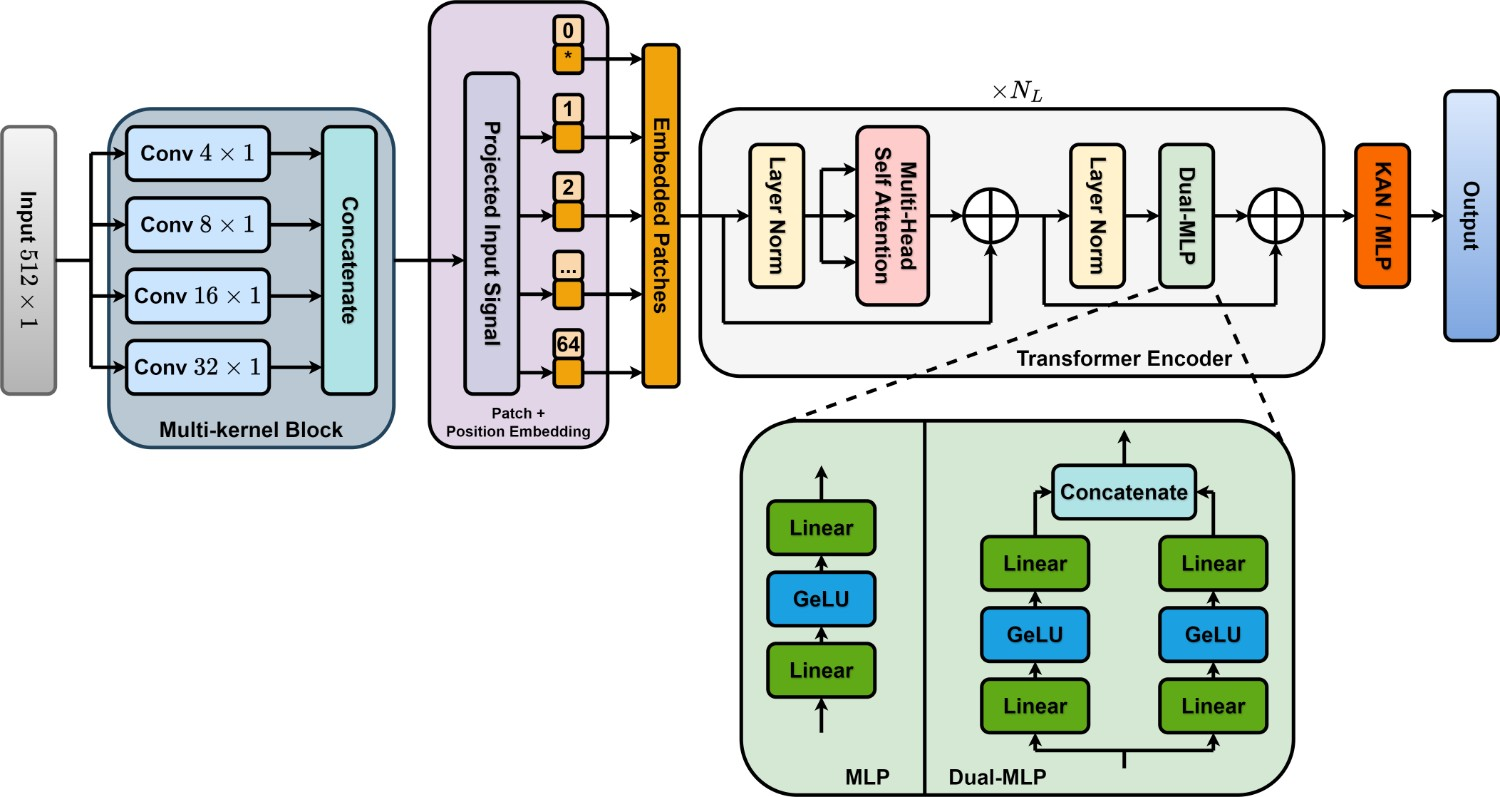
\includegraphics[width=\linewidth]{figs/OverallArchitecture.png}
\caption{Kiến trúc mô hình SMART-NIR}
\label{fig:smartnir}
\end{figure}

\subsubsection{Khối Multi-kernel}

Phổ NIR đầu vào được biểu diễn dưới dạng vector $\mathbf{X} \in \mathbb{R}^{L \times C}$,
với $L$ là độ dài phổ (số bước sóng) và $C = 1$ là số kênh. Khối Multi-kernel
gồm bốn nhánh tích chập song song với kích thước nhân lần lượt là
$4 \times 1$, $8 \times 1$, $16 \times 1$ và $32 \times 1$, cho phép trích
xuất đặc trưng thô ở nhiều tỉ lệ khác nhau. Ở nhánh thứ $i$ ($i \in
\{1,2,3,4\}$), một nhân tích chập $\mathbf{W}_i$ có kích thước $K_i =
(C_{out}, K_w, K_h)$ -- với $C_{out}$ là số kênh đầu ra, $K_w$ và $K_h$ lần
lượt là chiều rộng và chiều cao của nhân -- được áp dụng lên $\mathbf{X}$
với bước nhảy chung $S = (4,1)$ và đệm $P_i$ riêng cho từng nhánh:
\begin{align}
\mathbf{F}_1 &= \mathrm{Conv}\big(\mathbf{X}, \mathbf{W}_1, K_1{=}(C_{out},4,1), S, P_1{=}(0,0)\big) \notag\\
\mathbf{F}_2 &= \mathrm{Conv}\big(\mathbf{X}, \mathbf{W}_2, K_2{=}(C_{out},8,1), S, P_2{=}(3,0)\big) \notag\\
\mathbf{F}_3 &= \mathrm{Conv}\big(\mathbf{X}, \mathbf{W}_3, K_3{=}(C_{out},16,1), S, P_3{=}(7,0)\big) \notag\\
\mathbf{F}_4 &= \mathrm{Conv}\big(\mathbf{X}, \mathbf{W}_4, K_4{=}(C_{out},32,1), S, P_4{=}(15,0)\big)
\label{eq:multikernel}
\end{align}
Bốn đặc trưng thô $\mathbf{F}_1, \mathbf{F}_2, \mathbf{F}_3, \mathbf{F}_4$
được nối theo chiều kênh, tạo thành đầu ra $\mathbf{X}_0$ của khối
Multi-kernel.

\subsubsection{Patch + Position Embedding}

Đặc trưng thô $\mathbf{X}_0$ được chuyển vị và làm phẳng theo chiều không
gian để tạo thành chuỗi token, sau đó nối với một token phân loại học được
$\mathbf{x}_{cls}$ và cộng thêm embedding vị trí học được $\mathbf{E}_{pos}$,
tạo thành chuỗi đầu vào $\mathbf{X}_1$ cho khối mã hóa Transformer:
\begin{equation}
\mathbf{X}_1 = \mathrm{Concat}\big(\mathbf{x}_{cls}, \mathbf{X}_0^{T}\big) + \mathbf{E}_{pos}
\label{eq:posemb}
\end{equation}

\subsubsection{Khối mã hóa Transformer}

Khối mã hóa Transformer nắm bắt các phụ thuộc phức tạp trong chuỗi token
thông qua một chồng lớp, mỗi lớp gồm cơ chế tự chú ý đa đầu (Multi-Head
Self-Attention -- MHSA) nối tiếp một mạng truyền thẳng (feedforward), có
chuẩn hóa lớp (Layer Normalization) trước mỗi khối và kết nối tắt (skip
connection) để giảm hiện tượng tiêu biến gradient.

\textbf{Tự chú ý đa đầu:} Từ chuỗi đầu vào $\mathbf{X}_1 \in
\mathbb{R}^{(H_{out}+1)\times C_{out}}$ ($H_{out}$ là số token thô, chưa
tính token phân loại), ba ma trận Query, Key, Value được tạo ra bằng phép
chiếu tuyến tính học được: $\mathbf{Q} = \mathbf{X}_1 \mathbf{W}_Q$,
$\mathbf{K} = \mathbf{X}_1 \mathbf{W}_K$, $\mathbf{V} = \mathbf{X}_1
\mathbf{W}_V$, với $\mathbf{W}_Q$, $\mathbf{W}_K$, $\mathbf{W}_V$ là các ma
trận trọng số có thể học. Trọng số chú ý giữa mỗi cặp token được tính bằng
tích vô hướng chuẩn hóa giữa $\mathbf{Q}$ và $\mathbf{K}$, qua hàm softmax để
phản ánh mức độ quan trọng tương đối của từng token trong chuỗi:
\begin{equation}
SA(\mathbf{X}_1) = \mathrm{softmax}\!\left(\mathbf{Q}\mathbf{K}^{T}/\sqrt{H_{out}+1}\right)\mathbf{V}
\label{eq:sa}
\end{equation}
Cơ chế MHSA mở rộng tự chú ý (self-attention) chuẩn bằng cách thực hiện
$N_h$ phép tính chú ý song song, gọi là các đầu chú ý (head); mỗi đầu chiếu
tuyến tính riêng để nắm bắt một khía cạnh quan hệ khác nhau trong dữ liệu,
rồi các đầu ra được nối lại và biến đổi tuyến tính để tạo kết quả cuối cùng:
\begin{align}
MHSA(\mathbf{X}_1) = \mathrm{Concat}\big(&SA_1(\mathbf{X}_1), SA_2(\mathbf{X}_1), \notag\\
&\dots, SA_{N_h}(\mathbf{X}_1)\big)
\label{eq:mhsa}
\end{align}

\textbf{Dual-MLP:} Để giảm chi phí tính toán mà vẫn duy trì, thậm chí cải
thiện hiệu năng, token đầu ra $\mathbf{z}$ của khối MHSA được tách theo
chiều cuối thành hai nửa bằng nhau $\mathbf{m}$ và $\mathbf{n}$, mỗi nửa đi
qua một nhánh biến đổi tuyến tính riêng biệt rồi nối lại:
\begin{align}
\mathrm{DUAL\text{-}MLP} = \mathrm{Concat}\big(&\mathbf{W}_{fc4}\,\mathrm{GELU}(\mathbf{W}_{fc2}\,\mathbf{m}), \notag\\
&\mathbf{W}_{fc3}\,\mathrm{GELU}(\mathbf{W}_{fc1}\,\mathbf{n})\big)
\label{eq:dualmlp}
\end{align}
với $\mathbf{W}_{fc1}, \mathbf{W}_{fc2}, \mathbf{W}_{fc3}, \mathbf{W}_{fc4}$
là các ma trận trọng số học được của bốn nhánh tuyến tính minh họa ở
Hình~\ref{fig:smartnir}. Việc xử lý song song hai nửa đặc trưng theo cách
này giúp mô hình học được các mẫu đặc trưng đa dạng hơn mà không làm phát
sinh chi phí tính toán đáng kể.

\subsubsection{Bộ phân loại / hồi quy}

Ở đầu ra, kiến trúc KAN đóng vai trò bộ phân loại hoặc hồi quy, với hai lớp
ẩn kích thước giảm dần (32, 16), như minh họa ở Hình~\ref{fig:kan}. Khác với
MLP truyền thống dùng trọng số tuyến tính cho mỗi kết nối, KAN thay thế các
ma trận trọng số bằng các hàm một biến có thể học được, áp dụng độc lập theo
từng chiều của đầu vào.

\begin{figure}[htbp]
\centering
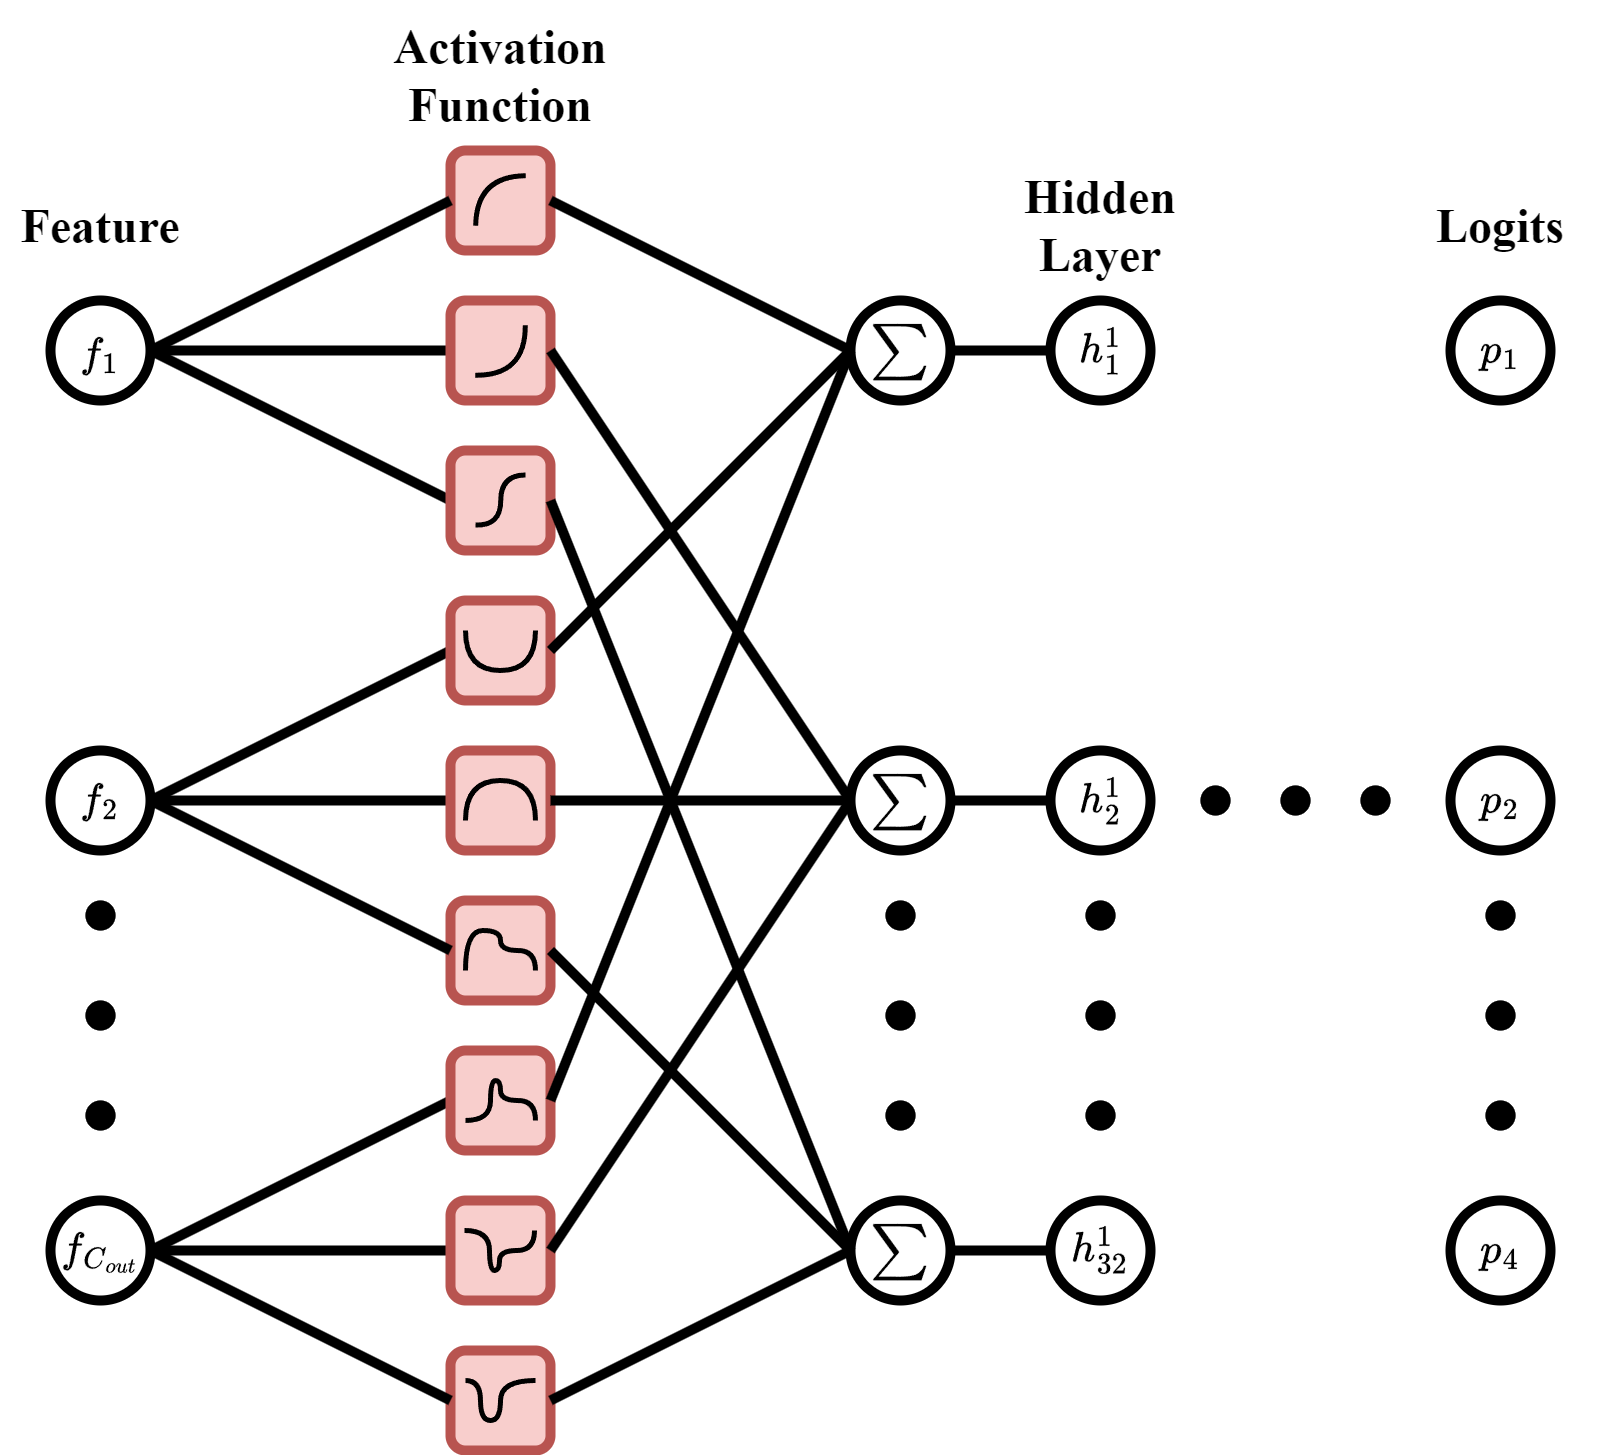
\includegraphics[width=\linewidth]{figs/KAN.png}
\caption{Kiến trúc mô hình KAN}
\label{fig:kan}
\end{figure}

\subsection{Mô hình XGBoost}
\label{sec:xgboost}

XGBoost (Extreme Gradient Boosting) là thuật toán học tập hợp (ensemble
learning) thuộc họ Gradient Boosting Decision Trees (GBDT), được phát triển
để khắc phục các
hạn chế của Gradient Boosting truyền thống về hiệu năng, khả năng mở rộng và
độ ổn định trên dữ liệu lớn, phức tạp -- nhờ đó trở thành một trong những
phương pháp phổ biến nhất cho bài toán phân loại và hồi quy.

Cốt lõi của XGBoost là ý tưởng tăng cường tuần tự (boosting): một tập hợp
cây quyết định (weak learners) được huấn luyện tuần tự, mỗi cây mới học để
bù đắp sai lệch mà các
cây trước đó chưa dự đoán tốt, thay vì huấn luyện độc lập như bagging. Gọi
$y_i$ và $\hat{y}_i$ lần lượt là nhãn thực và giá trị dự đoán của mẫu $i$,
hàm mục tiêu được tối ưu ở mỗi vòng lặp có dạng
\begin{equation}
L = \sum_i l\big(y_i, \hat{y}_i\big) + \sum_k \Omega(f_k),
\label{eq:xgb}
\end{equation}
trong đó $l(\cdot)$ là hàm mất mát đo độ sai lệch giữa $y_i$ và $\hat{y}_i$,
còn $\Omega(f_k)$ là số hạng điều chuẩn áp dụng cho cây thứ $k$ (ký hiệu
$f_k$), giúp kiểm soát độ phức tạp của cây và giảm nguy cơ quá khớp.

Khác với Gradient Boosting truyền thống chỉ dùng gradient bậc nhất, XGBoost
tận dụng khai triển Taylor bậc hai của hàm mất mát -- kết hợp cả gradient
(đạo hàm bậc 1) và Hessian (đạo hàm bậc 2) -- giúp ước lượng chính xác hơn
mức cải thiện khi thêm một cây mới, nhờ đó quá trình tối ưu hội tụ nhanh và
ổn định hơn. Mỗi cây được xây dựng theo hướng tham lam, với tiêu chí chia
nhánh dựa trên mức độ giảm của hàm mục tiêu, hỗ trợ cả chiến lược mở rộng
theo chiều sâu (depth-wise) lẫn mở rộng theo nút mang lại lợi ích lớn nhất
(leaf-wise), kèm cơ chế cắt tỉa dựa trên độ lợi (gain) để loại sớm các nhánh
không mang lại cải thiện đáng kể.

Nhờ sự cân bằng giữa độ chính xác, khả năng diễn giải và hiệu năng tính
toán, XGBoost được ứng dụng rộng rãi và đóng vai trò quan trọng trong hệ
sinh thái học máy hiện đại.

%=====================================================================
\section{Dữ liệu}

Bộ dữ liệu gồm phổ NIR thu từ hai máy quang phổ FLAMENIR và OCEANFX trên
chín loại rau củ quả phổ biến tại Việt Nam, kèm nhãn nồng độ (mg/kg; giá trị
$-1$ nghĩa là không phát hiện) của 19 loại thuốc trừ sâu, được xác định bằng
phương pháp phân tích hóa học chuyên sâu trong phòng thí nghiệm. Phần này
trình bày thống kê mô tả (EDA) trên từng máy: phân bố mẫu theo loại rau củ
quả, tỉ lệ nhiễm từng loại thuốc trừ sâu, đặc điểm phổ NIR theo từng loại, và
phân bố nồng độ trong các mẫu có phát hiện.

\subsection{Thống kê mô tả}
\label{sec:overview-stats}

\begin{table}[htbp]
\centering
\caption{Thông số chung của hai máy quang phổ}
\label{tab:overview-stats}
\footnotesize
\begin{tabular}{|l|r|r|}
\hline
\textbf{Thông số} & \textbf{FLAMENIR} & \textbf{OCEANFX} \\
\hline
Số lượng mẫu & 173.252 & 126.147\textsuperscript{*} \\
Số lượng bước sóng & 128 & 2.136 \\
Số lượng lớp phân loại & 9 & 9 \\
Số thuốc trừ sâu cần dự đoán & 19 & 19 \\
\hline
\end{tabular}

\vspace{2pt}
{\footnotesize \textsuperscript{*}đã loại 1 mẫu ngoại lai do lỗi cảm biến.}
\end{table}

Bảng~\ref{tab:overview-stats} cho thấy sự đánh đổi giữa hai máy: FLAMENIR
thu được nhiều mẫu hơn (173.252 so với 126.147) nhưng với độ phân giải phổ
thấp hơn nhiều (128 so với 2.136 điểm bước sóng) so với OCEANFX. Cả hai máy
đều khảo sát cùng 9 loại rau củ quả và 19 thuốc trừ sâu, cho phép so sánh
trực tiếp hiệu năng mô hình giữa hai cấu hình phần cứng khác nhau ở
Mục~\ref{sec:results}.

\begin{table}[htbp]
\centering
\caption{Số lượng mẫu theo loại rau củ quả}
\label{tab:cat-counts}
\footnotesize
\begin{tabular}{|l|r|r|}
\hline
\multirow{2}{*}{\textbf{Loại}} & \multicolumn{2}{c|}{\textbf{Số lượng mẫu}} \\
\cline{2-3}
 & \textbf{FLAMENIR} & \textbf{OCEANFX} \\
\hline
Khổ Qua      & 21.833 & 17.683 \\
Mồng Tơi     & 15.636 & 12.187 \\
Cải Thìa     & 21.269 & 16.905 \\
Cà Chua      & 16.672 & 12.289 \\
Cải Bẹ Xanh  & 15.691 & 15.916 \\
Dưa Leo      & 23.069 & 15.566 \\
Xà Lách      & 15.597 & 7.868 \\
Đậu Cove     & 20.334 & 16.256 \\
Cà Rốt       & 23.151 & 11.477 \\
\hline
\end{tabular}
\end{table}

Bảng~\ref{tab:cat-counts} cho thấy phân bố mẫu giữa các loại rau củ quả
không hoàn toàn cân bằng. Trên FLAMENIR, chênh lệch giữa loại nhiều mẫu nhất
(Cà Rốt, 23.151) và ít mẫu nhất (Xà Lách, 15.597) khoảng 1,5 lần; trên
OCEANFX, mức chênh lệch rõ rệt hơn, khoảng 2,2 lần giữa Khổ Qua (17.683) và
Xà Lách (7.868) -- Xà Lách là loại thiểu số trên cả hai máy. Mất cân bằng
này là một trong các lý do bài toán phân loại (Mục~\ref{sec:smartnir}) dùng
kiểm định chéo K-Fold phân tầng (Stratified K-Fold) và theo dõi cả
Precision/Recall/F1-score theo trung bình không trọng số qua các lớp
(macro-average) thay vì chỉ Accuracy.

\begin{table}[htbp]
\centering
\caption{Số lượng mẫu không chứa / có chứa từng thuốc trừ sâu}
\label{tab:sub-counts}
\footnotesize
\setlength{\tabcolsep}{4pt}
\resizebox{\linewidth}{!}{%
\begin{tabular}{|l|r|r|r|r|}
\hline
\multirow{2}{*}{\textbf{Thuốc trừ sâu}} & \multicolumn{2}{c|}{\textbf{FLAMENIR}} & \multicolumn{2}{c|}{\textbf{OCEANFX}} \\
\cline{2-5}
 & \textbf{Không chứa} & \textbf{Có chứa} & \textbf{Không chứa} & \textbf{Có chứa} \\
\hline
Thiamethoxam        & 159.315 & 13.937 & 114.054 & 12.093 \\
Permethrin          & 148.443 & 24.809 & 100.283 & 25.864 \\
Metalaxyl           & 169.091 & 4.161  & 121.745 & 4.402 \\
Azoxystrobin        & 160.518 & 12.734 & 115.526 & 10.621 \\
Imidaclopird        & 154.619 & 18.633 & 121.747 & 4.400 \\
Difenoconazole      & 160.624 & 12.628 & 115.807 & 10.340 \\
Cypermethrin        & 160.330 & 12.922 & 113.326 & 12.821 \\
Cyhalothrin         & 169.934 & 3.318  & 120.598 & 5.549 \\
Chlorantraniliprol  & 171.622 & 1.630  & 123.260 & 2.887 \\
Chlopyrifos Methyl  & 171.371 & 1.881  & 122.342 & 3.805 \\
Emamectin benzoate  & 160.062 & 13.190 & 125.115 & 1.032 \\
Chlorothalonil      & 158.417 & 14.835 & 117.761 & 8.386 \\
\rowcolor{red!12}Triadimefon         & 173.252 & 0      & 126.147 & 0 \\
\rowcolor{red!12}Cyantraniliprole    & 163.202 & 10.050 & 126.147 & 0 \\
\rowcolor{red!12}Flutolanil          & 173.252 & 0      & 126.147 & 0 \\
Indoxacarb          & 166.359 & 6.893  & 120.073 & 6.074 \\
Abamectin           & 162.971 & 10.281 & 119.094 & 7.053 \\
\rowcolor{red!12}Propamocarb.HCL     & 173.252 & 0      & 126.147 & 0 \\
Chlothianidin       & 166.446 & 6.806  & 120.073 & 6.074 \\
\hline
\end{tabular}%
}

\vspace{2pt}
{\footnotesize \colorbox{red!12}{\rule{0pt}{6pt}\rule{6pt}{0pt}} các dòng
tô đỏ: có ít nhất một máy với 0 mẫu dương (không thể huấn luyện mô hình
phát hiện/hồi quy tương ứng trên máy đó).}
\end{table}

Bảng~\ref{tab:sub-counts} cho thấy mức mất cân bằng lớp nghiêm trọng hơn
nhiều so với bài toán phân loại: đa số thuốc trừ sâu chỉ xuất hiện trong
dưới 10\% tổng số mẫu, với Permethrin là thuốc trừ sâu phổ biến nhất trên cả
hai máy (14,3\% ở FLAMENIR, 20,5\% ở OCEANFX). Ba thuốc trừ sâu (Triadimefon,
Flutolanil, Propamocarb.HCL) không có mẫu dương nào trên cả hai máy; riêng
Cyantraniliprole có 10.050 mẫu dương trên FLAMENIR nhưng bằng 0 trên OCEANFX,
phản ánh sự khác biệt giữa hai đợt lấy mẫu chứ không phải do bản thân thiết
bị đo. Các thuốc trừ sâu không có mẫu dương trên một máy nào đó khiến không
thể huấn luyện được mô hình phát hiện/hồi quy tương ứng, thể hiện qua các
giá trị NaN ở Mục~\ref{sec:results}.

\subsection{Trực quan hóa dữ liệu}

\begin{figure*}[t]
\centering
\begin{subfigure}[b]{0.49\textwidth}
\centering
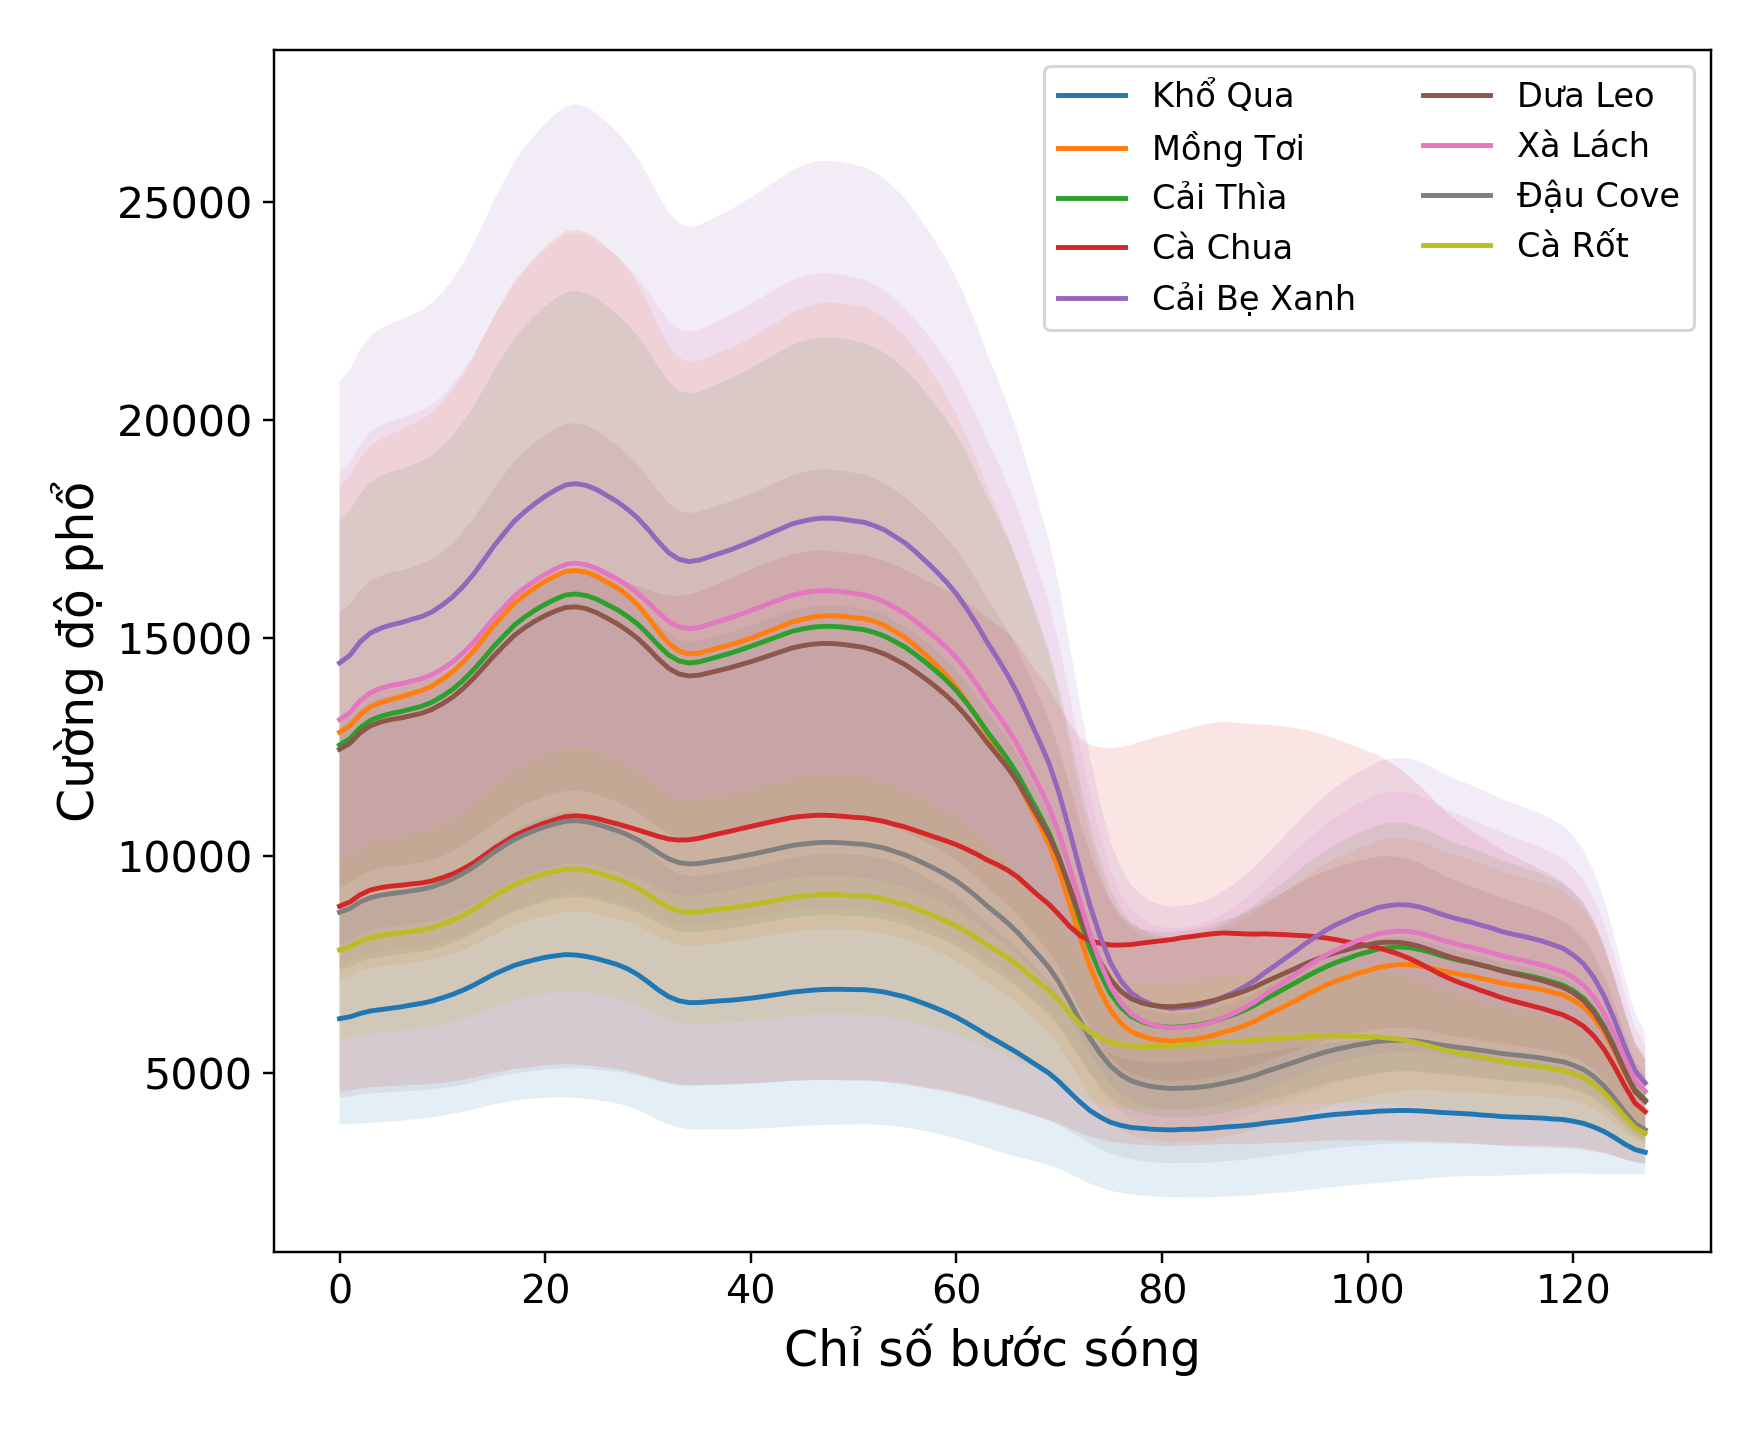
\includegraphics[width=\textwidth]{figs/spectra_FLAMENIR.png}
\caption{Máy FLAMENIR}
\label{fig:spectra-flamenir}
\end{subfigure}
\hfill
\begin{subfigure}[b]{0.49\textwidth}
\centering
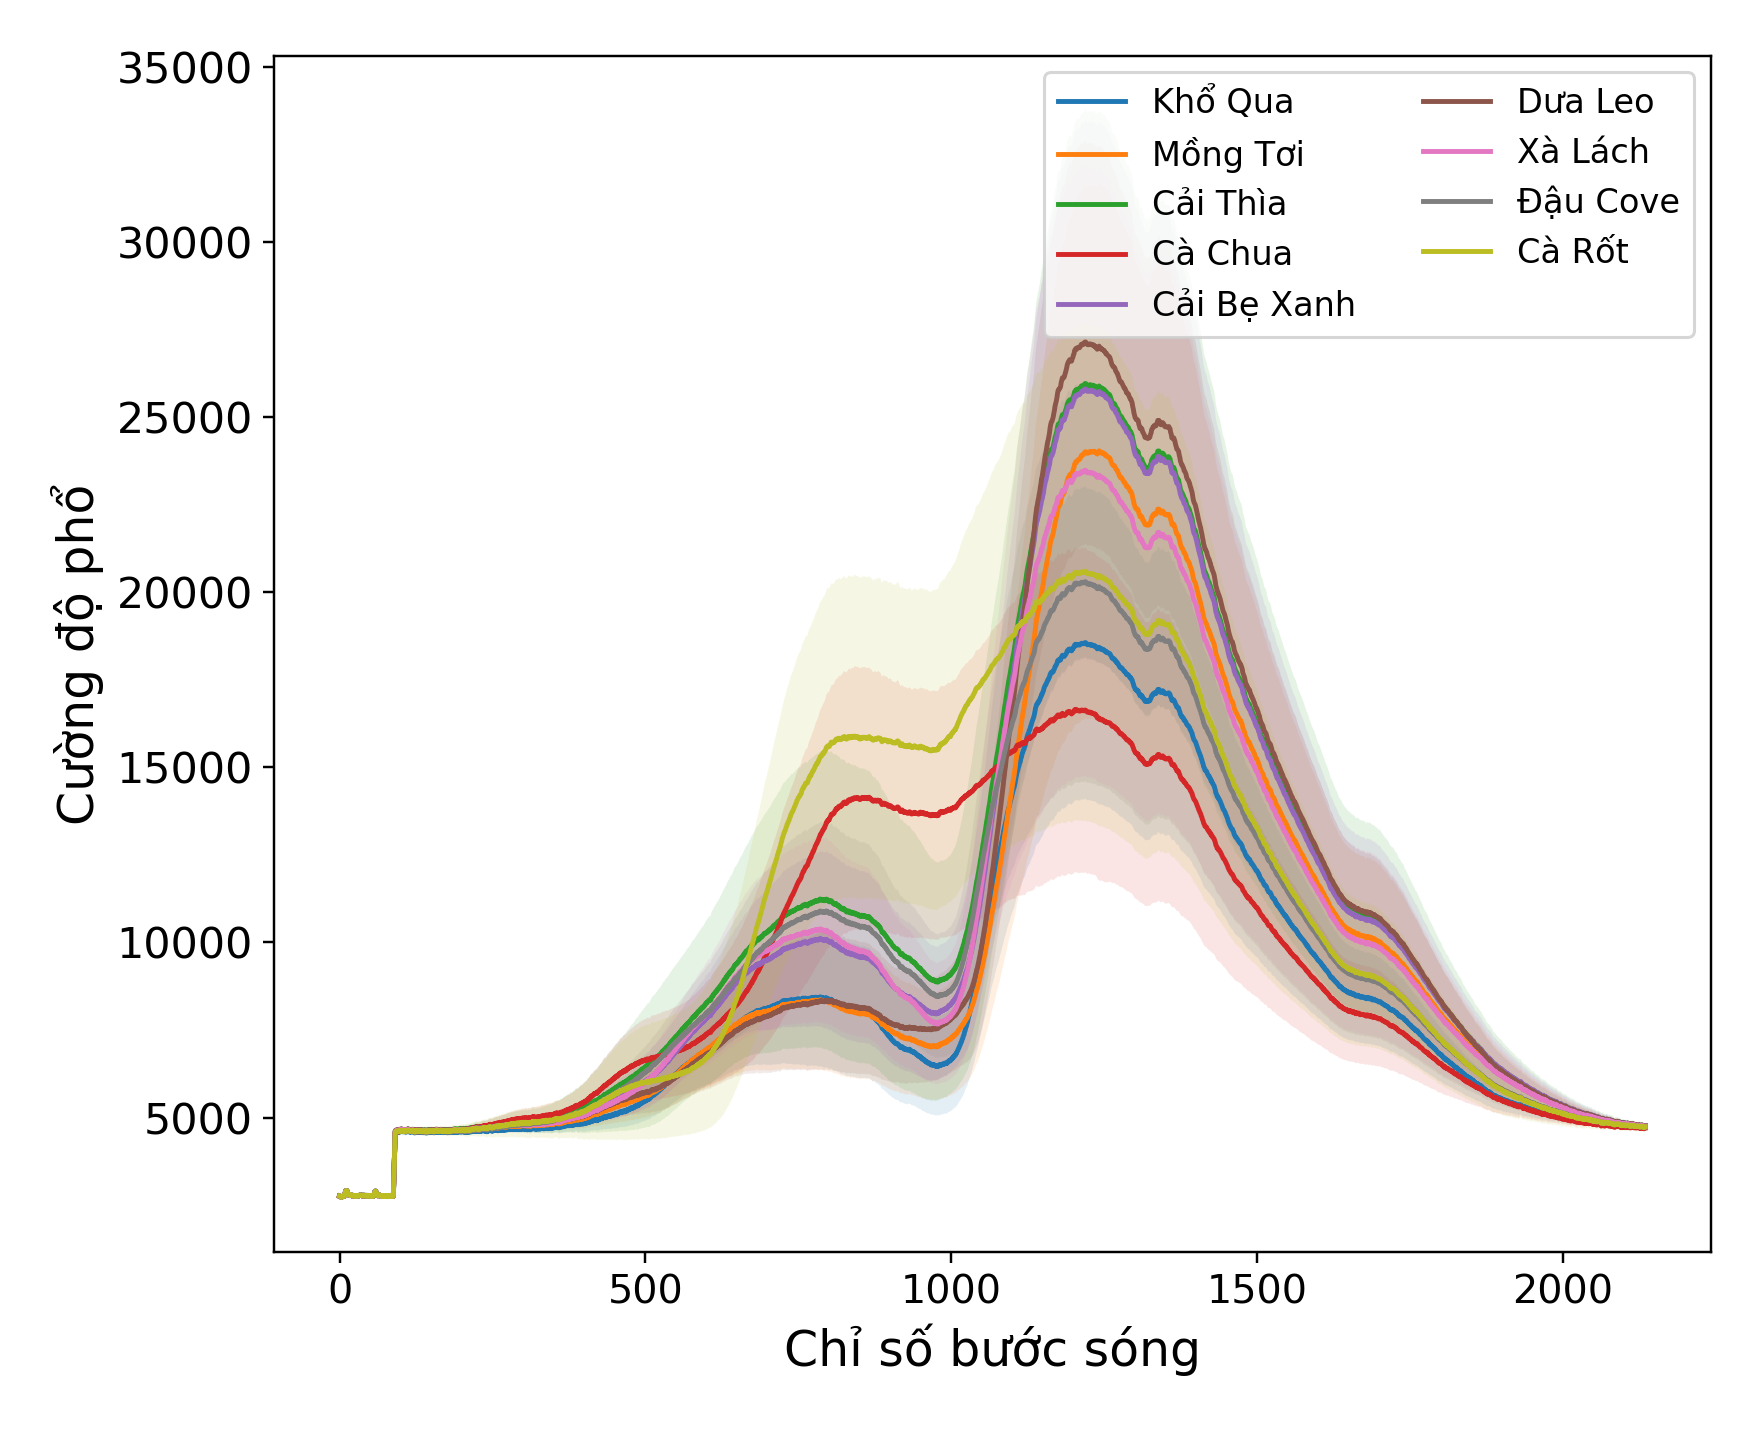
\includegraphics[width=\textwidth]{figs/spectra_OCEANFX.png}
\caption{Máy OCEANFX}
\label{fig:spectra-oceanfx}
\end{subfigure}
\caption{Phổ NIR trung bình (đường liền) và dải độ lệch chuẩn (vùng tô) theo
loại rau củ quả}
\label{fig:spectra}
\end{figure*}

Hình~\ref{fig:spectra} cho thấy các loại rau củ quả có hình dạng phổ NIR khá
tương đồng trên cùng một máy (cùng vị trí đỉnh hấp thụ) nhưng khác nhau rõ
rệt về cường độ tuyệt đối -- ở FLAMENIR, Cải Bẹ Xanh và Xà Lách cho cường độ
cao nhất còn Khổ Qua thấp nhất; đây là cơ sở để mô hình phân biệt được loại
rau củ quả từ phổ thô. Phổ từ OCEANFX (Hình~\ref{fig:spectra-oceanfx}) có độ
phân giải bước sóng cao hơn nhiều (2.136 so với 128 điểm) và bộc lộ rõ hai
đỉnh hấp thụ chính, cùng dải độ lệch chuẩn rộng hơn ở vùng bước sóng thấp,
phản ánh mức biến thiên tín hiệu cao hơn giữa các cá thể mẫu trong vùng này.

\begin{figure*}[t]
\centering
\begin{subfigure}[b]{0.49\textwidth}
\centering
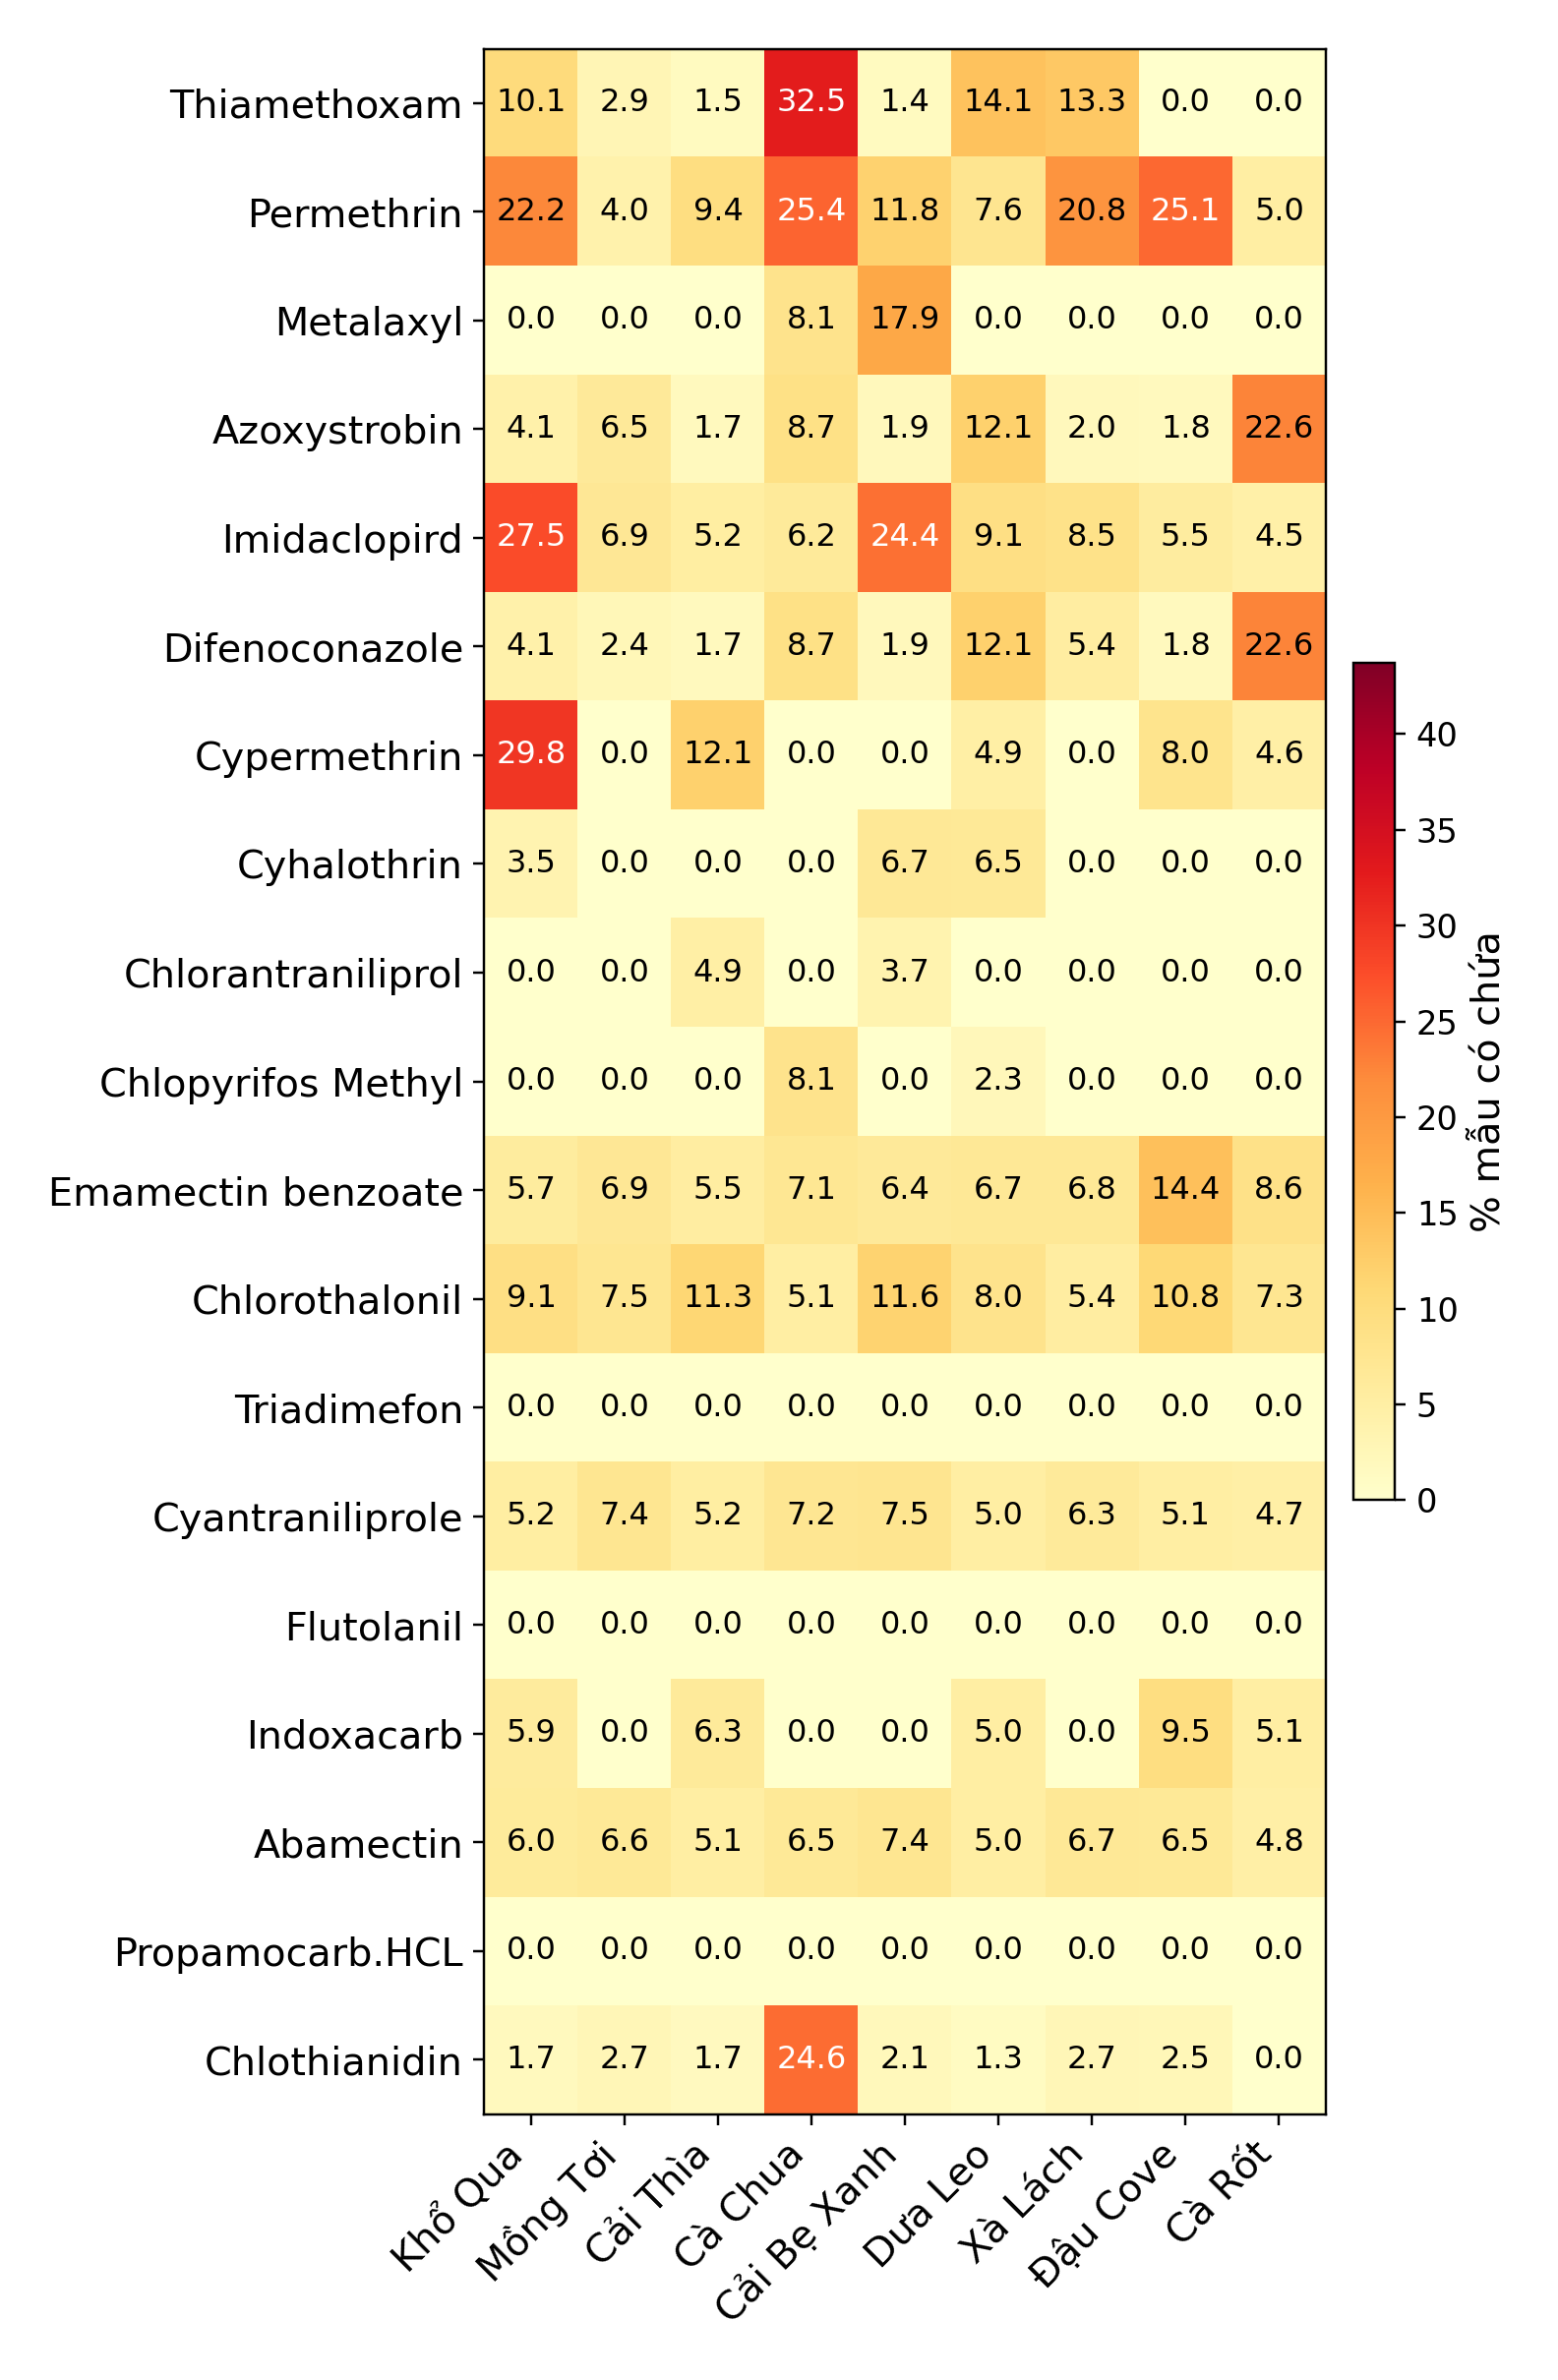
\includegraphics[width=\textwidth]{figs/crosstab_FLAMENIR.png}
\caption{Máy FLAMENIR}
\label{fig:crosstab-flamenir}
\end{subfigure}
\hfill
\begin{subfigure}[b]{0.49\textwidth}
\centering
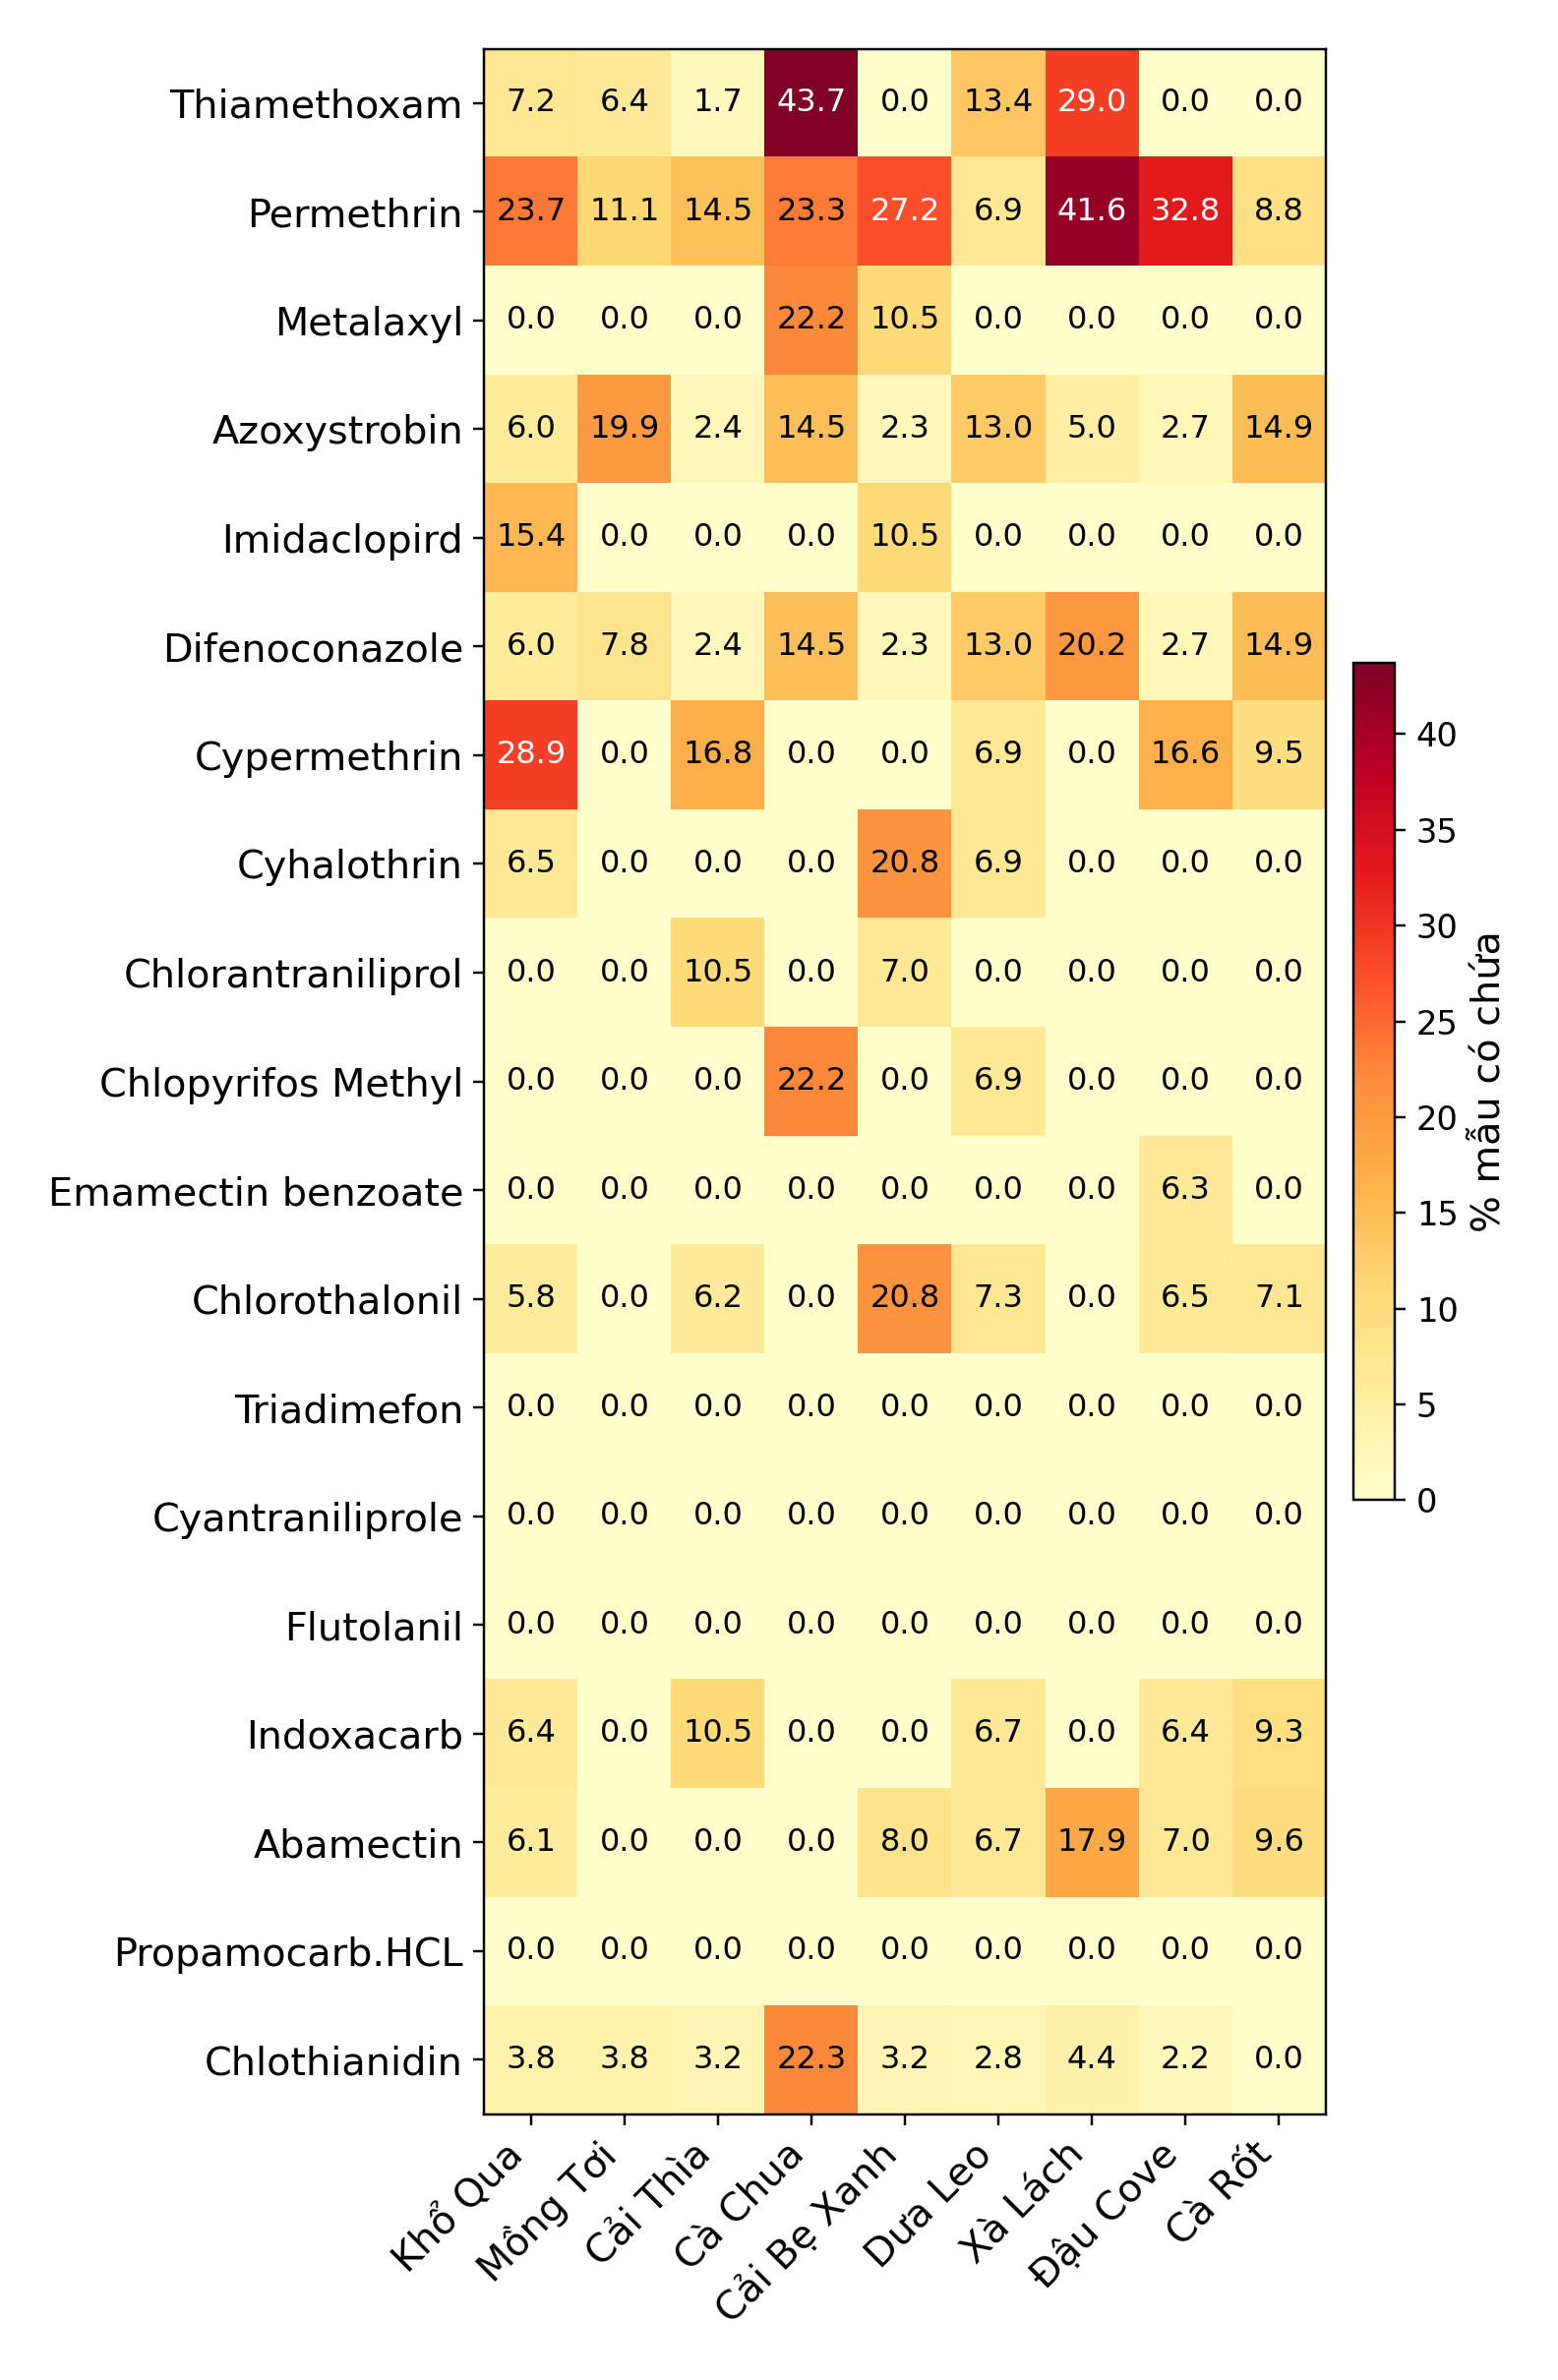
\includegraphics[width=\textwidth]{figs/crosstab_OCEANFX.png}
\caption{Máy OCEANFX}
\label{fig:crosstab-oceanfx}
\end{subfigure}
\caption{Tỉ lệ (\%, một chữ số thập phân) mẫu có chứa từng thuốc trừ sâu
theo loại rau củ quả, dùng chung thang màu giữa hai máy để so sánh}
\label{fig:crosstab}
\end{figure*}

Hình~\ref{fig:crosstab} cho thấy tỉ lệ nhiễm phân bố không đồng đều giữa các
loại rau củ quả và giữa hai máy: ở FLAMENIR, Cà Chua có tỉ lệ nhiễm
Thiamethoxam và Chlothianidin cao nhất trong khi Khổ Qua nổi bật với
Cypermethrin và Imidaclopird; ở OCEANFX, ô có tỉ lệ nhiễm cao nhất toàn bảng
là Thiamethoxam tại Cà Chua (43,7\%), theo sau là Permethrin tại Xà Lách
(41,6\%) -- Permethrin cũng là thuốc trừ sâu phổ biến nhất trên máy này, với
tỉ lệ trên 20\% ở nhiều loại rau củ quả khác nhau.

\begin{figure*}[t]
\centering
\begin{subfigure}[b]{0.49\textwidth}
\centering
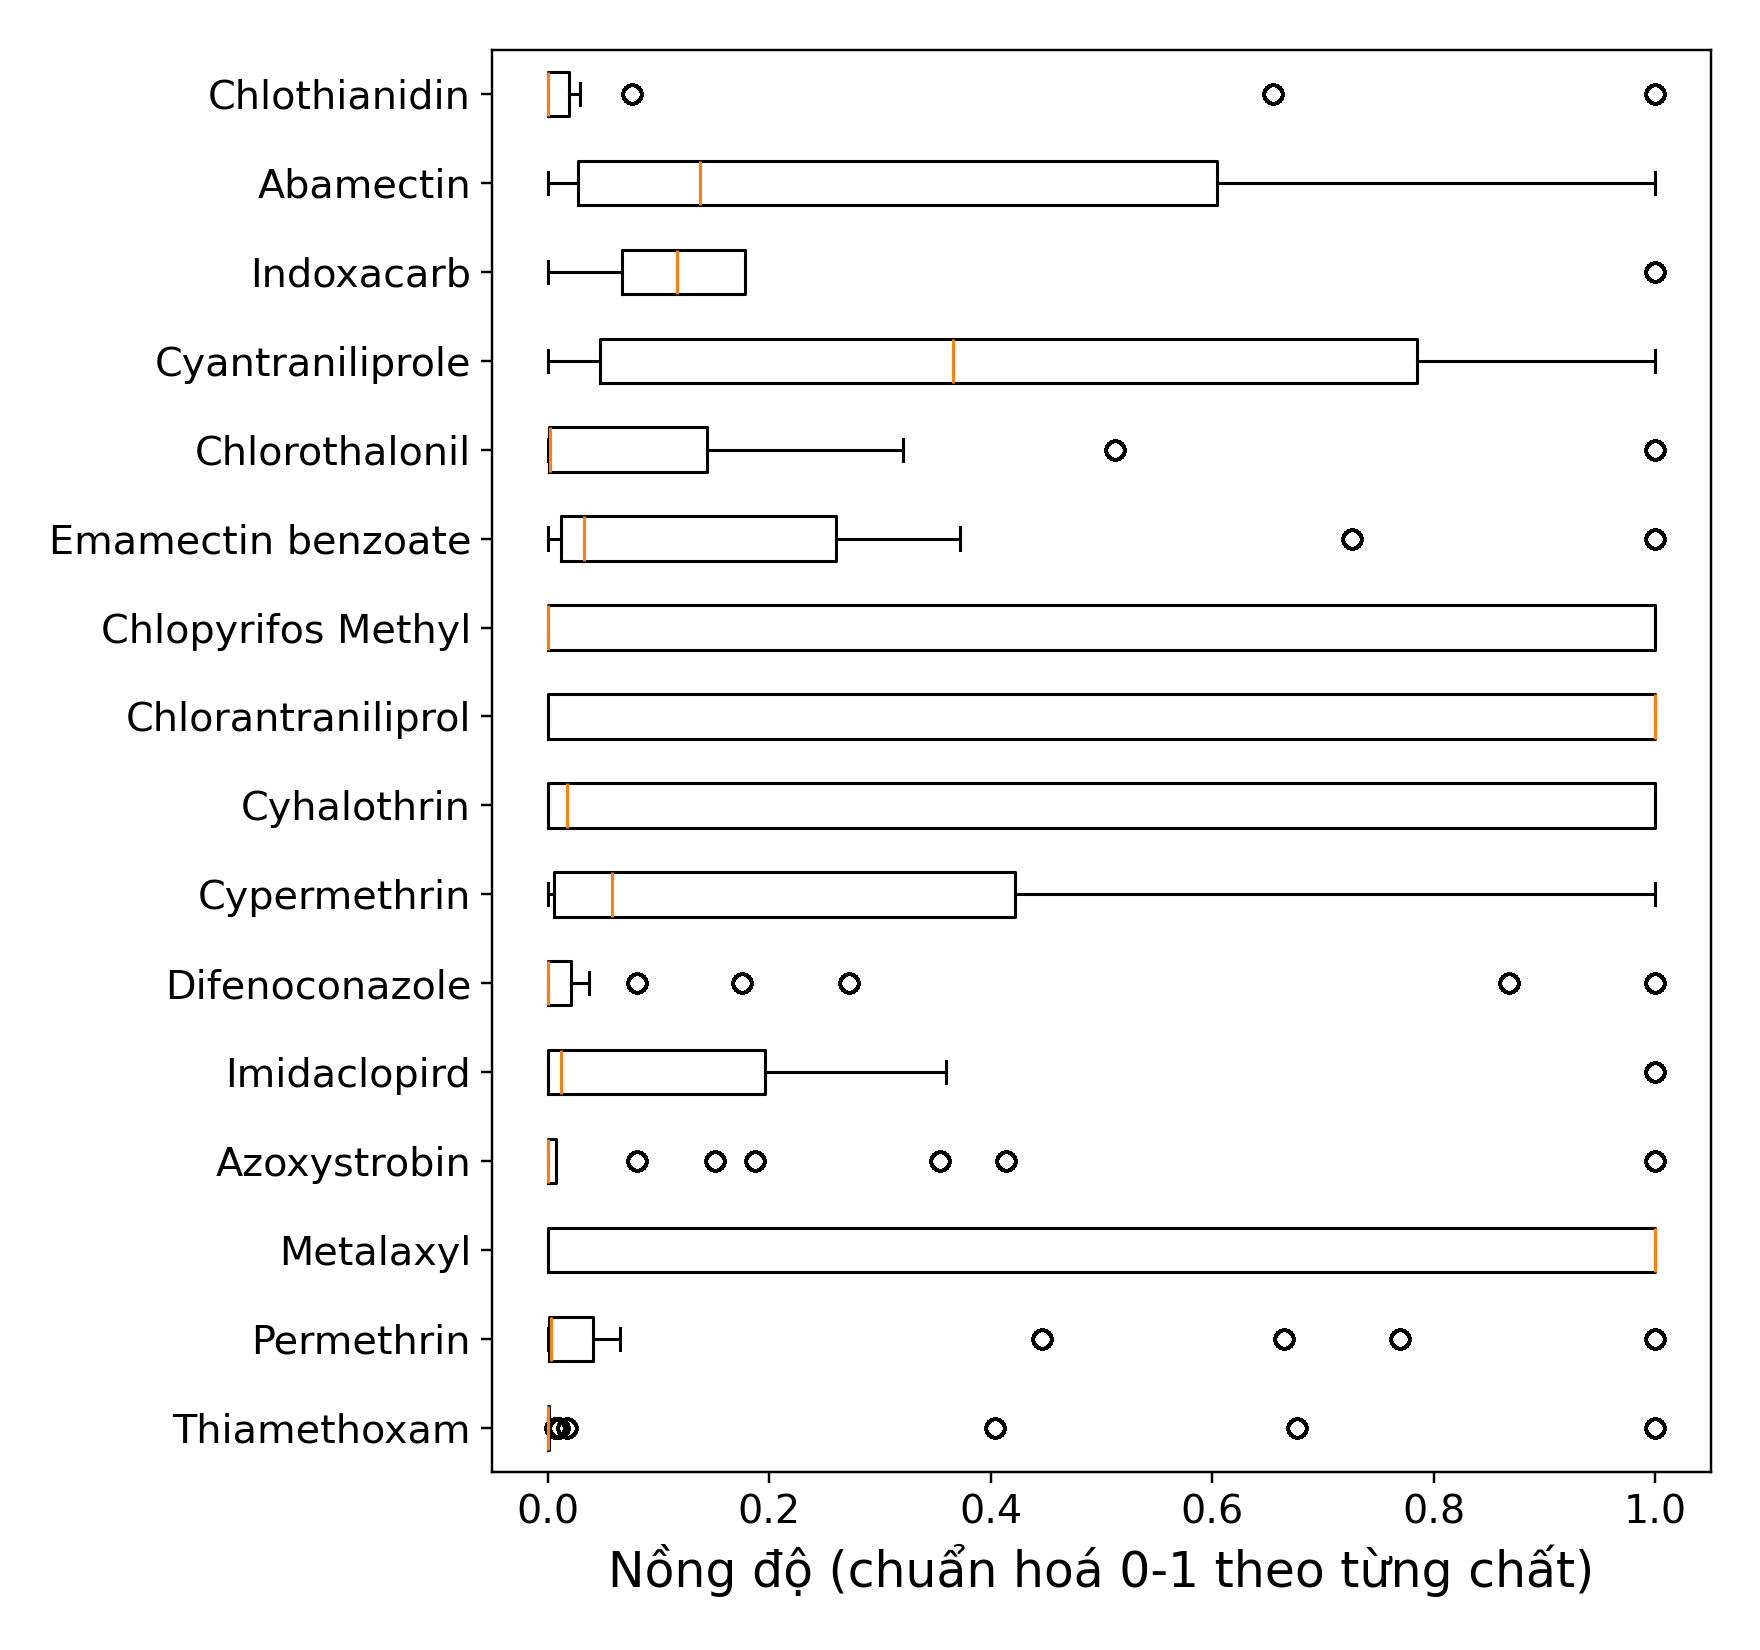
\includegraphics[width=\textwidth]{figs/concbox_FLAMENIR.png}
\caption{Máy FLAMENIR}
\label{fig:concbox-flamenir}
\end{subfigure}
\hfill
\begin{subfigure}[b]{0.49\textwidth}
\centering
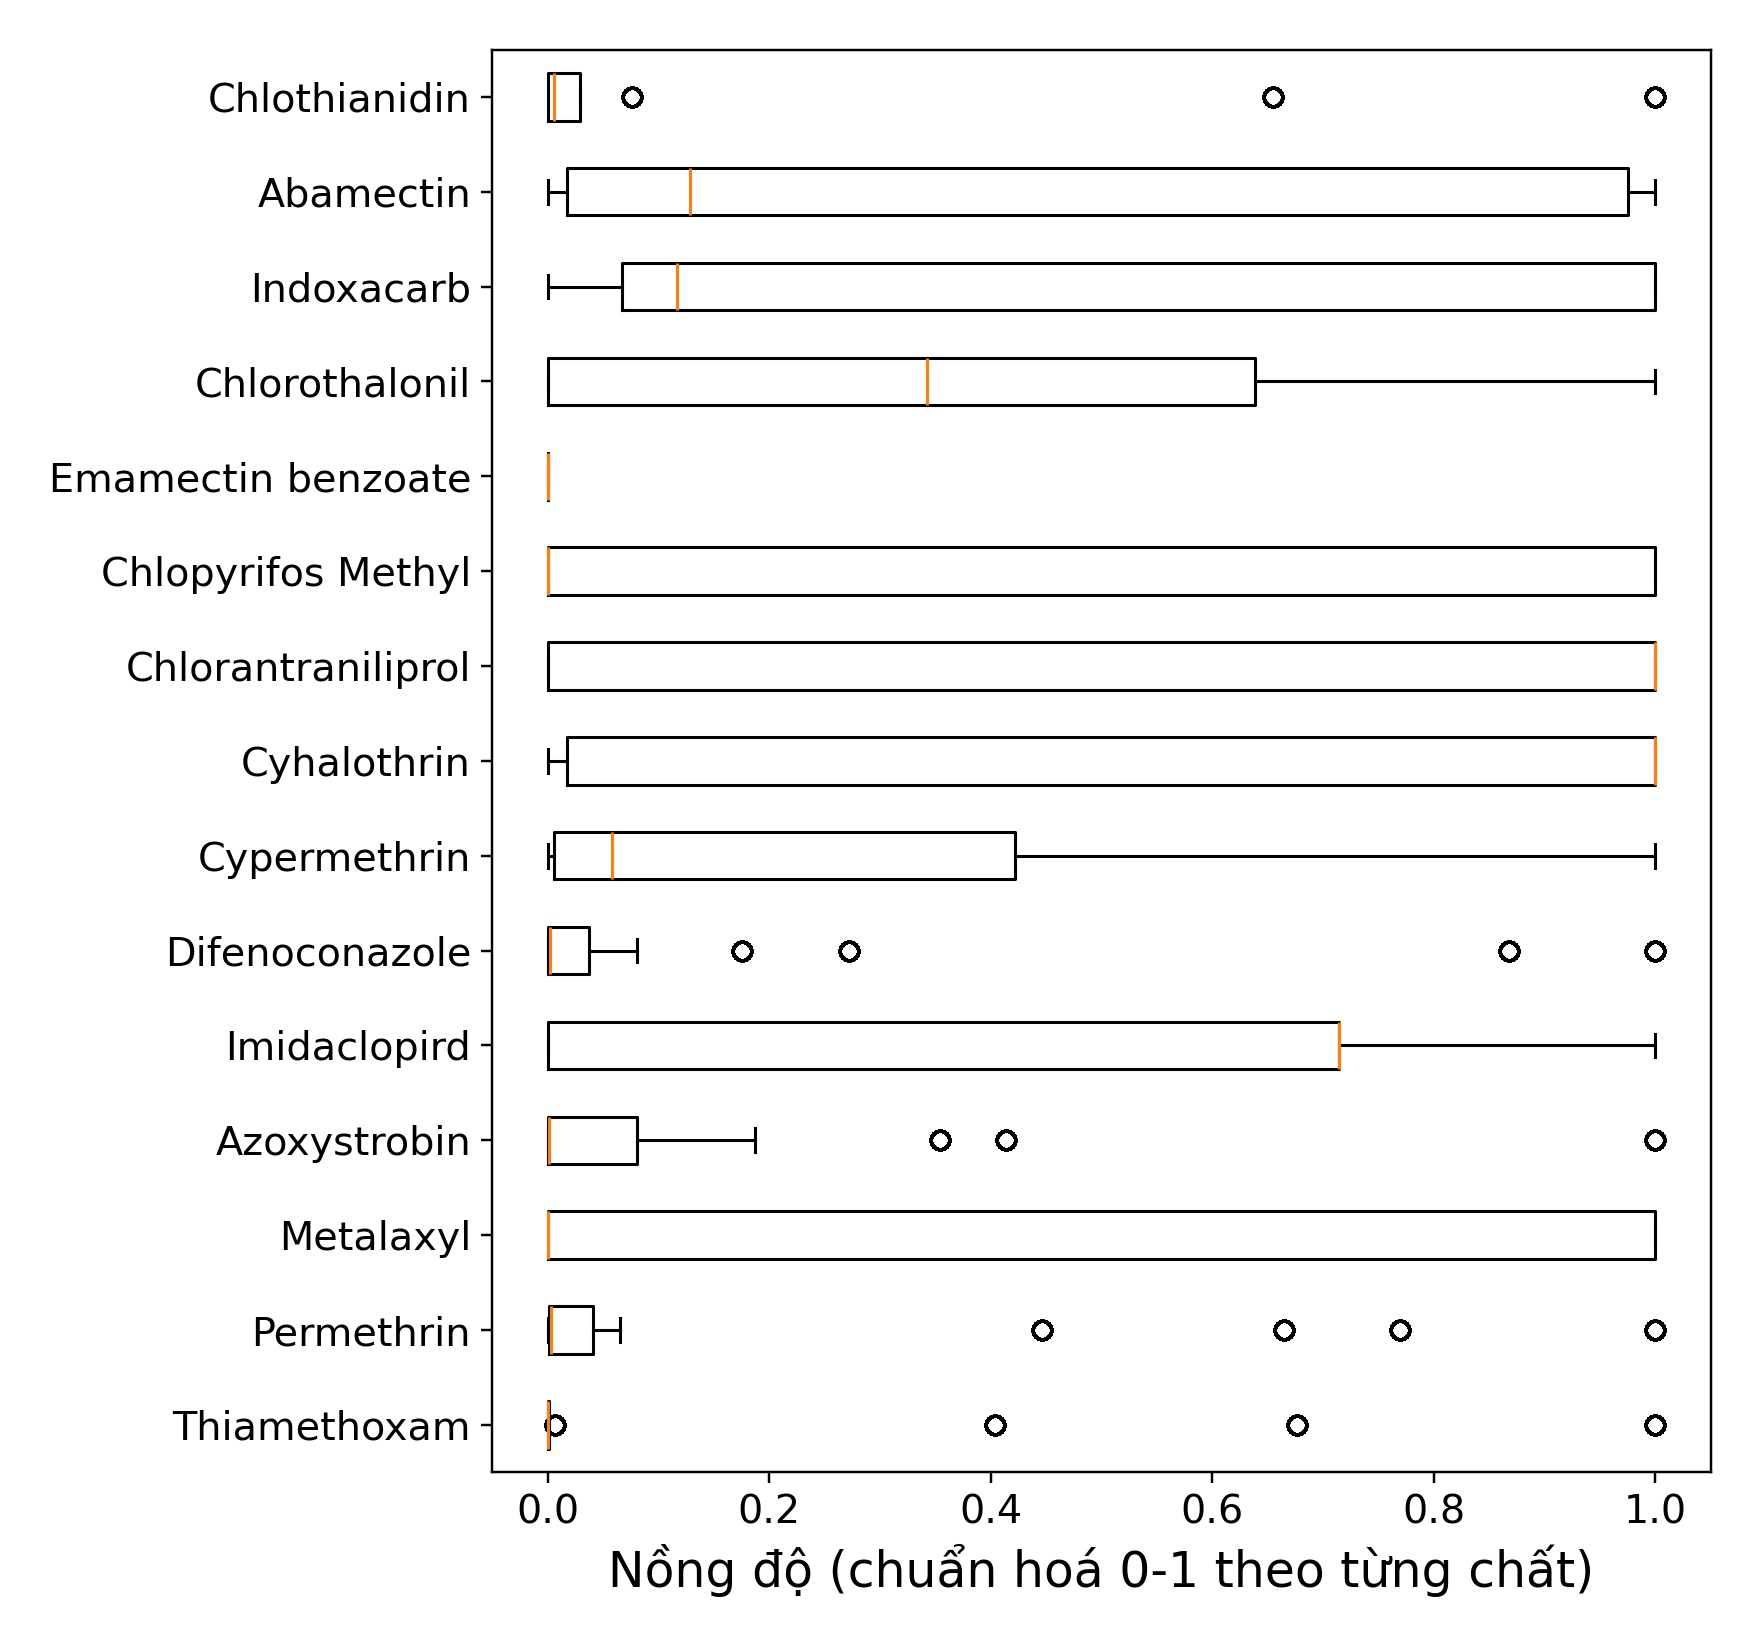
\includegraphics[width=\textwidth]{figs/concbox_OCEANFX.png}
\caption{Máy OCEANFX}
\label{fig:concbox-oceanfx}
\end{subfigure}
\caption{Phân bố nồng độ (chuẩn hóa 0--1 theo từng chất) trong các mẫu có
phát hiện}
\label{fig:concbox}
\end{figure*}

Về mức độ đồng nhiễm: trong tổng số 173.252 mẫu FLAMENIR, 47.635 mẫu
(27,5\%) không phát hiện thuốc trừ sâu nào (mẫu sạch), 96.021 mẫu (55,4\%)
chỉ chứa đúng một loại, và 29.596 mẫu (17,1\%) đồng thời chứa từ hai loại trở
lên -- trong đó 563 mẫu chứa cùng lúc cả bốn loại. Ở OCEANFX, trong tổng số
126.147 mẫu, 47.047 mẫu (37,3\%) là mẫu sạch, 51.266 mẫu (40,7\%) chứa đúng
một loại, và 27.834 mẫu (22,1\%) đồng thời chứa từ hai loại trở lên -- trong
đó 1.003 mẫu chứa cả bốn loại. Tỉ lệ đồng nhiễm ở OCEANFX cao hơn FLAMENIR
(22,1\% so với 17,1\%), một khác biệt cần lưu ý khi so sánh hiệu năng phát
hiện giữa hai máy ở Mục~\ref{sec:results}. Đồng nhiễm nhiều thuốc trừ sâu
cũng là một trong những lý do khiến việc tách bài toán phát hiện thành 19 mô
hình nhị phân độc lập (Mục~\ref{sec:xgboost}) phù hợp hơn một bộ phân loại đa
nhãn đơn lẻ giả định các nhãn độc lập tuyệt đối.

%=====================================================================
\section{Thiết lập thực nghiệm}

Tất cả các thí nghiệm được thực hiện trên hệ điều hành Ubuntu 22.04, sử dụng
PyTorch 2.9.1 và Python 3.12.11 với CUDA hỗ trợ, chạy trên GPU NVIDIA RTX
5090 Ti và được trang bị CPU Intel\textregistered{} Xeon\textregistered{}
E5-2696 v3 @ 2.30 GHz.

\subsection{Phân loại rau củ quả}

\subsubsection{Tiền xử lý dữ liệu}

Dữ liệu phổ NIR thường chịu ảnh hưởng của nhiễu, tán xạ và sai lệch đường
nền, do đó cần được tiền xử lý trước khi đưa vào mô hình phân loại. Trước
hết, dữ liệu được làm sạch nhằm loại bỏ các phổ lỗi và giá trị ngoại lai.
Tiếp theo, kỹ thuật Savitzky--Golay được sử dụng để giảm nhiễu và hiệu chỉnh
đường nền giúp làm nổi bật các đặc trưng quan trọng.

Để hạn chế ảnh hưởng của tán xạ ánh sáng, phương pháp chuẩn hóa biến số
chuẩn (Standard Normal Variate -- SNV) được sử dụng. Sau đó, dữ liệu được
chuẩn hóa về cùng thang đo nhằm đảm bảo quá trình học ổn định. Cuối cùng, dữ
liệu được chia thành các tập huấn luyện và kiểm tra phục vụ cho bài toán
phân loại.

\subsubsection{Chi tiết huấn luyện}
\label{sec:clf-training}

Quá trình huấn luyện mô hình phân loại phổ NIR được triển khai bằng PyTorch,
với chiến lược kiểm định chéo K-Fold nhằm đánh giá độ ổn định và khả năng
tổng quát hóa của mô hình. Cụ thể, dữ liệu được chia thành 5 fold theo
phương pháp K-Fold phân tầng (Stratified K-Fold), đảm bảo phân bố nhãn giữa
các tập huấn luyện và kiểm tra được giữ cân bằng.

Trước mỗi fold, dữ liệu huấn luyện được sử dụng để ước lượng tham số chuẩn
hóa và ánh xạ nhãn, sau đó áp dụng thống nhất cho cả tập huấn luyện và tập
kiểm tra nhằm tránh rò rỉ thông tin. Trong mỗi fold, dữ liệu được lấy mẫu và
gom thành lô (batch) kích thước 512, giúp tăng hiệu quả huấn luyện trên GPU.

Mô hình SMART-NIR được khởi tạo với các tham số chính bao gồm: (1) Chiều dài
tín hiệu đầu vào bằng độ dài phổ sau tiền xử lý; (2) Số kênh đầu ra cho mỗi
nhánh đa kernel là 64; (3) Kích thước không gian đặc trưng là 128; (4) Số
tầng Transformer là 3 với 4 đầu tự chú ý mỗi tầng; (5) Bộ phân loại
cuối sử dụng KAN với số lớp đầu ra tương ứng với số nhãn trong tập dữ liệu.

Hàm mất mát được sử dụng là Focal Loss ($\gamma = 2$), với trọng số $\alpha$
của mỗi lớp tỉ lệ nghịch với tần suất lớp đó trong fold huấn luyện. So với
hàm entropy chéo (Cross-Entropy) thông thường, Focal Loss giảm đóng góp
gradient của các mẫu dễ (thường thuộc lớp đa số) và tập trung hơn vào lớp
thiểu số, phù hợp với đặc điểm mất cân bằng dữ liệu đã nêu ở
Mục~\ref{sec:overview-stats}. Quá trình tối ưu tham số được thực hiện bằng
trình tối ưu AdamW (suy giảm trọng số/weight decay $10^{-4}$) nhằm hạn chế
quá khớp (overfitting). Tốc độ học được điều chỉnh theo lịch trình gồm hai
giai đoạn: khởi động (warmup) tuyến tính trong 10 lượt huấn luyện đầu
(epoch, 5\% tổng số lượt), tăng dần từ $10^{-4}$ lên $10^{-3}$, sau đó giảm
dần về gần 0 theo lịch suy giảm dạng cos (Cosine Annealing) trong các lượt
còn lại. Trong mỗi lượt huấn luyện, mô hình được huấn luyện trên tập huấn
luyện với cơ chế lan truyền ngược, sau đó được đánh giá trên tập đánh giá ở
chế độ suy luận theo các tiêu chí trình bày ở Mục~\ref{sec:metrics}. Cơ chế
dừng sớm (early stopping) được áp dụng dựa trên độ chính xác trên tập đánh
giá, với ngưỡng kiên nhẫn là 10 epoch: mô hình đạt độ chính xác kiểm tra cao
nhất sẽ được lưu lại, và quá trình huấn luyện dừng sớm nếu không có cải
thiện trong nhiều epoch liên tiếp.

\subsection{Dự đoán hàm lượng các thuốc trừ sâu có trong mẫu}

\subsubsection{Tiền xử lý dữ liệu}
\label{sec:stage2-preprocess}

Tương tự với quy trình tiền xử lý ở bài toán phân loại, dữ liệu phổ NIR ban
đầu được làm sạch nhằm loại bỏ các phổ lỗi và giá trị ngoại lai, sau đó áp
dụng Savitzky--Golay và SNV để làm nổi bật các đặc trưng quan trọng và hạn
chế ảnh hưởng của tán xạ ánh sáng.

Toàn bộ dữ liệu (kể cả mất cân bằng) được giữ nguyên, không loại bớt mẫu
không chứa thuốc trừ sâu, nhằm không lãng phí thông tin từ các mẫu âm; mất
cân bằng nhãn được xử lý trực tiếp trong quá trình huấn luyện XGBoost
(Mục~\ref{sec:xgboost}, Bước 1) thông qua trọng số
\texttt{scale\_pos\_weight}. Đối với bài toán hồi quy nồng độ
(Bước 2), biến mục tiêu được biến đổi log ($\log(1+y)$) trước khi chuẩn hóa
Z-score theo từng fold, nhằm giảm độ lệch phải của phân bố nồng độ (đa số
giá trị nhỏ, một số ít giá trị lớn) và ổn định quá trình học; các chỉ số
MAE, RMSE, $R^{2}$ báo cáo ở Mục~\ref{sec:results} được tính sau khi biến
đổi ngược dự đoán về đơn vị nồng độ gốc (mg/kg). Cuối cùng, dữ liệu được
chia thành các tập huấn luyện và kiểm tra phục vụ cho bài toán phát hiện và
dự đoán hàm lượng thuốc trừ sâu có trong mẫu.

\subsubsection{Chi tiết huấn luyện}
\label{sec:stage-training}

Một chiến lược huấn luyện hai bước được sử dụng nhằm xử lý hiệu quả bài toán
phân tích phổ NIR với nhiều thuốc trừ sâu khác nhau. Cách tiếp cận này cho phép
tách biệt rõ ràng giữa bài toán phát hiện sự hiện diện của thuốc trừ sâu và bài
toán ước lượng nồng độ, từ đó nâng cao độ ổn định và độ chính xác của toàn hệ
thống.

\textbf{Bước 1:} Ở bước đầu tiên, mỗi thuốc trừ sâu được xem như một bài toán
phân loại nhị phân độc lập, trong đó mục tiêu là xác định liệu thuốc trừ sâu đó
có xuất hiện trong mẫu hay không. Nhãn được xây dựng bằng cách ánh xạ giá trị
đo: các mẫu có giá trị lớn hơn 0 được gán nhãn 1 (có thuốc trừ sâu), trong khi
các mẫu có giá trị $-1$ được gán nhãn 0 (không có thuốc trừ sâu). Quá trình huấn
luyện sử dụng kiểm định chéo K-Fold phân tầng (5 fold) để đảm bảo phân bố
nhãn cân bằng giữa các tập.

Mô hình được huấn luyện bằng XGBoost với hàm mục tiêu binary logistic, kết
hợp cơ chế dừng sớm dựa trên log-loss của tập kiểm tra. Trọng số
\texttt{scale\_pos\_weight} được đặt bằng tỉ lệ số mẫu âm/dương của fold
huấn luyện để bù đắp mất cân bằng nhãn mà không cần loại bỏ dữ liệu (như đã
nêu ở Mục~\ref{sec:stage2-preprocess}). Độ phức tạp cây (số cây, độ sâu tối
đa, tốc độ học) được điều chỉnh theo số mẫu dương của từng thuốc trừ sâu --
thuốc có ít mẫu dương hơn dùng cây nông và ít cây hơn để giảm nguy cơ quá
khớp.

Vì \texttt{scale\_pos\_weight} làm lệch xác suất đầu ra của mô hình khỏi xác
suất thực, một bước hiệu chỉnh Platt scaling (hồi quy logistic một chiều)
được fit trên chính dự đoán của tập huấn luyện, rồi áp dụng lại cho tập kiểm
tra để tránh rò rỉ thông tin.

Thay vì cố định ngưỡng phân loại ở 0,5, ngưỡng quyết định được chọn tự động
bằng cách quét toàn bộ đường cong Precision-Recall (trên xác suất đã hiệu
chỉnh của \emph{tập huấn luyện}, cùng lý do tránh rò rỉ như bước hiệu chỉnh
Platt scaling) và chọn ngưỡng cho Precision cao nhất trong số các ngưỡng đạt
Recall lớp dương $\geq 0{,}9$; nếu không ngưỡng nào đạt được mục tiêu này,
ngưỡng cho Recall cao nhất được dùng thay thế. Lựa chọn này phản ánh đặc thù
bài toán an toàn thực phẩm, nơi bỏ sót một mẫu thực sự có thuốc trừ sâu
(false negative) gây hậu quả nghiêm trọng hơn nhiều so với một cảnh báo giả
(false positive) cần kiểm tra lại. Ngưỡng được lưu lại cùng mô hình và bộ
hiệu chỉnh để tái sử dụng khi suy luận.

Sau khi huấn luyện, mô hình được đánh giá theo các tiêu chí phân loại ở
Mục~\ref{sec:metrics}, cùng với PR-AUC và Brier score trước/sau hiệu chỉnh
để theo dõi thêm chất lượng xác suất dự đoán; do ngưỡng được tối ưu theo
Recall thay vì mặc định 0,5, PR-AUC (không phụ thuộc ngưỡng) là chỉ số đáng
tin cậy hơn Accuracy/F1 khi so sánh hiệu năng phát hiện giữa các thuốc trừ
sâu.

Bước này đóng vai trò như một bộ lọc (screening stage), giúp loại bỏ các mẫu
không chứa thuốc trừ sâu trước khi thực hiện hồi quy nồng độ.

\textbf{Bước 2:} Ở bước thứ hai, chỉ các mẫu có giá trị nồng độ hợp lệ (khác
$-1$) mới được sử dụng để huấn luyện mô hình hồi quy. Với mỗi thuốc trừ sâu, một
mô hình SMART-NIR riêng biệt được huấn luyện nhằm dự đoán chính xác giá trị
nồng độ từ phổ NIR.

Dữ liệu được chia theo K-Fold phân tầng (5 fold) trên các nhóm phân vị
(quantile bin) của nồng độ mục tiêu, giúp mỗi fold có phân bố nồng độ tương
đồng nhau thay vì lệch ngẫu nhiên như K-Fold thường; với thuốc trừ sâu không
đủ dữ liệu để chia nhóm phân vị, phương pháp tự động chuyển về K-Fold thường.
Trước mỗi fold, tham số chuẩn hóa của phổ và của biến mục tiêu đã qua biến
đổi log (Mục~\ref{sec:stage2-preprocess}) được ước lượng từ tập huấn luyện
và áp dụng thống nhất cho tập kiểm tra. Mô hình SMART-NIR được cấu hình với
kiến trúc Transformer đa kernel và bộ hồi quy KAN ở đầu ra.

Quá trình huấn luyện sử dụng Mean Squared Error (MSE), tính trên biến mục
tiêu đã chuẩn hóa, làm hàm mất mát, cùng Adam optimizer với tốc độ học ban
đầu $10^{-3}$. Để cải thiện khả năng hội tụ, ReduceLROnPlateau được áp dụng
nhằm điều chỉnh tốc độ học dựa trên giá trị hàm mất mát trên tập đánh giá.
Đồng thời, cơ chế dừng sớm được sử dụng để tránh quá khớp.

Mô hình đạt giá trị hàm mất mát trên tập đánh giá (không gian đã chuẩn hóa)
thấp nhất trong mỗi fold sẽ được lưu lại, cùng với lịch sử huấn luyện và các
biểu đồ đánh giá. Các chỉ số MAE, RMSE và $R^{2}$ báo cáo ở
Mục~\ref{sec:results} được tính theo các tiêu chí ở Mục~\ref{sec:metrics},
sau khi biến đổi ngược dự đoán và nhãn thực về đơn vị nồng độ gốc để phản
ánh đúng sai số thực tế thay vì sai số trên không gian đã chuẩn hóa.

%=====================================================================
\section{Kết quả}
\label{sec:results}

\subsection{Tiêu chí đánh giá}
\label{sec:metrics}

Hiệu năng mô hình được đánh giá bằng bộ chỉ số phù hợp với từng loại bài
toán: phân loại (loại thực phẩm, Mục~\ref{sec:smartnir}; phát hiện thuốc trừ
sâu, Mục~\ref{sec:xgboost}) và hồi quy (dự đoán nồng độ, Bước 2 của
Mục~\ref{sec:xgboost}).

\textbf{Chỉ số phân loại.} Gọi $C$ là số lớp; với mỗi lớp $c$, gọi $TP_c$,
$FP_c$, $FN_c$ lần lượt là số mẫu dương thật, dương giả và âm giả của lớp đó
trên tập kiểm tra. Accuracy là tỉ lệ mẫu dự đoán đúng trên tổng số mẫu,
trong khi Precision, Recall và F1-score được tính theo trung bình không
trọng số qua các lớp (macro-average) để không bị chi phối bởi lớp đa số,
phù hợp với đặc điểm mất cân bằng dữ liệu đã nêu ở
Mục~\ref{sec:overview-stats}:
\begin{align}
\mathrm{Precision}_c = \frac{TP_c}{TP_c + FP_c}, \quad
\mathrm{Recall}_c = \frac{TP_c}{TP_c + FN_c}, \notag\\
F1_c = \frac{2 \cdot \mathrm{Precision}_c \cdot \mathrm{Recall}_c}{\mathrm{Precision}_c + \mathrm{Recall}_c}
\label{eq:prf1}
\end{align}
\begin{align}
\mathrm{Precision} &= \frac{1}{C}\sum_{c=1}^{C}\mathrm{Precision}_c, \notag\\
\mathrm{Recall} &= \frac{1}{C}\sum_{c=1}^{C}\mathrm{Recall}_c, \notag\\
F1 &= \frac{1}{C}\sum_{c=1}^{C}F1_c
\label{eq:macro}
\end{align}
Với bài toán phát hiện thuốc trừ sâu (Bước 1, nhị phân), $C=2$.

\textbf{Chỉ số bổ sung cho Bước 1.} Vì Bước 1 huấn luyện trên dữ liệu mất
cân bằng với trọng số \texttt{scale\_pos\_weight} (Mục~\ref{sec:xgboost}),
hai chỉ số bổ sung được theo dõi cùng Accuracy/Precision/Recall/F1: PR-AUC
(diện tích dưới đường cong Precision-Recall khi quét ngưỡng phân loại), ít
nhạy với mất cân bằng lớp hơn ROC-AUC; và Brier score -- sai số bình phương
trung bình giữa xác suất dự đoán $\hat{p}_i$ và nhãn thực $l_i \in \{0,1\}$,
$\mathrm{Brier} = \frac{1}{n}\sum_{i=1}^{n}(\hat{p}_i - l_i)^2$ -- đo chất
lượng hiệu chỉnh xác suất, được báo cáo trước và sau bước Platt scaling để
định lượng mức cải thiện.

\textbf{Chỉ số hồi quy.} Với $n$ mẫu trong tập kiểm tra, $y_i$ và $\hat{y}_i$
lần lượt là nồng độ thực và nồng độ dự đoán của mẫu $i$, và $\bar{y}$ là
nồng độ thực trung bình trên tập kiểm tra, hiệu năng hồi quy được đo bằng
MAE, RMSE và hệ số xác định $R^{2}$:
\begin{align}
\mathrm{MAE} &= \frac{1}{n}\sum_{i=1}^{n}\left|y_i - \hat{y}_i\right|, \notag\\
\mathrm{RMSE} &= \sqrt{\frac{1}{n}\sum_{i=1}^{n}\left(y_i - \hat{y}_i\right)^2}, \notag\\
R^{2} &= 1 - \frac{\sum_{i=1}^{n}\left(y_i - \hat{y}_i\right)^2}{\sum_{i=1}^{n}\left(y_i - \bar{y}\right)^2}
\label{eq:regmetrics}
\end{align}
MAE và RMSE càng nhỏ và $R^{2}$ càng gần 1 thể hiện mô hình dự đoán nồng độ
càng chính xác.

\subsection{Máy FLAMENIR}

\subsubsection{Phân loại rau củ quả}

\begin{table}[htbp]
\centering
\caption{Kết quả phân loại rau củ quả -- máy FLAMENIR}
\label{tab:flamenir-clf}
\footnotesize
\resizebox{\linewidth}{!}{%
\begin{tabular}{|l|c|c|c|c|}
\hline
\textbf{Fold} & \textbf{Accuracy} & \textbf{Precision} & \textbf{Recall} & \textbf{F1-Score} \\
\hline
Fold 1 & 95,17\% & 94,79\% & 94,81\% & 94,80\% \\
Fold 2 & 94,77\% & 94,33\% & 94,37\% & 94,35\% \\
Fold 3 & 92,49\% & 91,86\% & 91,97\% & 91,89\% \\
Fold 4 & 93,16\% & 92,59\% & 92,64\% & 92,60\% \\
Fold 5 & 94,34\% & 93,91\% & 93,98\% & 93,94\% \\
\hline
\textbf{Trung bình} & \textbf{93,98$_{\pm 1,01}$\%} & \textbf{93,50$_{\pm 1,10}$\%} & \textbf{93,55$_{\pm 1,07}$\%} & \textbf{93,51$_{\pm 1,10}$\%} \\
\hline
\end{tabular}%
}
\end{table}

Độ chính xác dao động từ 92,49\% (Fold 3) đến 95,17\% (Fold 1), chênh lệch
khoảng 2,7 điểm \% giữa các fold -- mức dao động vừa phải, cho thấy mô hình
khá ổn định qua các cách chia dữ liệu khác nhau. Precision và Recall luôn
sát nhau ở mọi fold, phù hợp với việc dùng Focal Loss cùng trọng số theo tần
suất lớp (Mục~\ref{sec:clf-training}) để cân bằng ảnh hưởng giữa 9 loại rau
củ quả.

\subsubsection{Dự đoán hàm lượng các thuốc trừ sâu có trong mẫu}

\textbf{a/ Phát hiện thuốc trừ sâu}

Ngưỡng quyết định (\texttt{threshold}) của mỗi fold được chọn tự động nhằm
đạt Recall lớp dương $\geq 0{,}9$ với Precision cao nhất có thể, thay vì cố
định ở 0,5 (chi tiết ở Mục~\ref{sec:stage-training}) -- phù hợp hơn với bài
toán an toàn thực phẩm, nơi bỏ sót một mẫu có thuốc trừ sâu thật (false
negative) nguy hiểm hơn một cảnh báo giả (false positive). Vì vậy Accuracy
và F1 (theo macro-average, tính trên cả hai lớp) không còn là chỉ số chính
để đánh giá -- PR-AUC (không phụ thuộc ngưỡng) phản ánh đúng hơn khả năng
phân biệt của mô hình.

\begin{table}[htbp]
\centering
\caption{Kết quả phát hiện thuốc trừ sâu (trung bình 5-fold) -- máy FLAMENIR}
\label{tab:flamenir-detect}
\footnotesize
\setlength{\tabcolsep}{2.5pt}
\resizebox{\linewidth}{!}{%
\begin{tabular}{|l|c|c|c|c|c|c|}
\hline
\textbf{Thuốc trừ sâu} & \textbf{Ngưỡng} & \textbf{Acc.} & \textbf{Prec.} & \textbf{Recall} & \textbf{F1} & \textbf{PR-AUC} \\
\hline
Thiamethoxam & 0,154 & 90,66\% & 71,52\% & 84,16\% & 75,80\% & 0,630 \\
Permethrin & 0,105 & 72,84\% & 63,68\% & 75,55\% & 63,73\% & 0,482 \\
Metalaxyl & 0,285 & 97,61\% & 74,66\% & 81,77\% & 77,73\% & 0,627 \\
Azoxystrobin & 0,086 & 87,27\% & 65,97\% & 82,64\% & 69,95\% & 0,529 \\
Imidaclopird & 0,117 & 83,60\% & 66,92\% & 80,21\% & 70,04\% & 0,521 \\
Difenoconazole & 0,088 & 87,61\% & 66,20\% & 82,77\% & 70,27\% & 0,533 \\
Cypermethrin & 0,129 & 88,29\% & 67,05\% & 82,31\% & 71,17\% & 0,521 \\
Cyhalothrin & 0,814 & 99,21\% & 95,52\% & 82,27\% & 87,72\% & 0,868 \\
Chlorantraniliprol & 0,678 & 99,29\% & 86,02\% & 70,08\% & 75,68\% & 0,571 \\
Chlopyrifos Methyl & 0,935 & 99,70\% & 98,96\% & 86,97\% & 92,07\% & 0,953 \\
Emamectin benzoate & 0,126 & 89,07\% & 67,77\% & 80,42\% & 71,66\% & 0,532 \\
Chlorothalonil & 0,163 & 89,47\% & 70,47\% & 83,11\% & 74,57\% & 0,570 \\
\rowcolor{red!12}Triadimefon & \multicolumn{6}{c|}{NaN (0 mẫu dương)} \\
Cyantraniliprole & 0,091 & 88,94\% & 64,16\% & 79,99\% & 68,09\% & 0,455 \\
\rowcolor{red!12}Flutolanil & \multicolumn{6}{c|}{NaN (0 mẫu dương)} \\
Indoxacarb & 0,201 & 95,43\% & 71,88\% & 82,52\% & 75,98\% & 0,591 \\
Abamectin & 0,088 & 89,74\% & 64,95\% & 78,61\% & 68,82\% & 0,481 \\
\rowcolor{red!12}Propamocarb.HCL & \multicolumn{6}{c|}{NaN (0 mẫu dương)} \\
Chlothianidin & 0,096 & 93,87\% & 67,23\% & 82,46\% & 72,03\% & 0,515 \\
\hline
\end{tabular}%
}
\end{table}

\textit{Ghi chú: NaN ứng với các thuốc trừ sâu không có mẫu dương nào trong
tập dữ liệu (cột FLAMENIR của Bảng \ref{tab:sub-counts}), nên không thể huấn
luyện được mô hình phát hiện/hồi quy.}

PR-AUC dao động khá rộng, từ 0,455 (Cyantraniliprole) đến 0,953 (Chlopyrifos
Methyl). Các chất có PR-AUC cao nhất (Chlopyrifos Methyl 0,953; Cyhalothrin
0,868) cũng là những chất được chọn ngưỡng quyết định cao hơn hẳn mức mặc
định 0,5 (lần lượt 0,935 và 0,814) -- vì mô hình đã tách biệt tốt hai lớp
ngay từ ngưỡng thấp, thuật toán có thể đẩy ngưỡng lên để tăng Precision mà
vẫn giữ Recall $\geq 0{,}9$. Phần lớn các chất còn lại có PR-AUC quanh mức
0,5--0,6 và ngưỡng thấp (0,08--0,2), đòi hỏi hạ ngưỡng sâu để đạt Recall mục
tiêu, kéo theo Precision giảm còn khoảng 64--75\% -- phản ánh đúng bản chất
khó của bài toán khi tín hiệu phổ NIR của các chất này chưa đủ đặc trưng để
phân biệt rạch ròi ở độ phân giải 128 bước sóng của FLAMENIR. Một ngoại lệ
đáng chú ý là Chlorantraniliprol: dù PR-AUC chỉ ở mức trung bình (0,571),
chất này vẫn được chọn ngưỡng khá cao (0,678), cho thấy đường cong
Precision-Recall của nó giữ Precision tốt cụ thể quanh điểm Recall $=0{,}9$
dù PR-AUC tổng thể (lấy trung bình trên toàn miền Recall) không cao.

\textbf{b/ Dự đoán hàm lượng}

\begin{table}[htbp]
\centering
\caption{Kết quả dự đoán hàm lượng (trung bình 5-fold) -- máy FLAMENIR}
\label{tab:flamenir-reg}
\footnotesize
\setlength{\tabcolsep}{2.5pt}
\begin{tabular}{|l|c|c|c|c|}
\hline
\textbf{Thuốc trừ sâu} & \textbf{MSE} & \textbf{MAE} & \textbf{RMSE} & \textbf{$R^2$ (\%)} \\
\hline
Thiamethoxam & 0,027 & 4,834 & 27,021 & 85,15 \\
Permethrin & 0,017 & 8,915 & 33,101 & 85,05 \\
\rowcolor{yellow!30}Metalaxyl & 0,001 & 0,000 & 0,001 & 99,63 \\
Azoxystrobin & 0,007 & 13,955 & 66,604 & 90,63 \\
Imidaclopird & 0,028 & 1,081 & 2,936 & 83,44 \\
Difenoconazole & 0,007 & 4,539 & 24,545 & 93,65 \\
Cypermethrin & 0,013 & 0,064 & 0,203 & 92,93 \\
\rowcolor{yellow!30}Cyhalothrin & 0,005 & 0,001 & 0,004 & 97,26 \\
\rowcolor{yellow!30}Chlorantraniliprol & 0,013 & 0,000 & 0,001 & 93,61 \\
\rowcolor{yellow!30}Chlopyrifos Methyl & 0,000 & 0,000 & 0,000 & 99,92 \\
Emamectin benzoate & 0,021 & 0,318 & 0,905 & 85,43 \\
Chlorothalonil & 0,015 & 401,527 & 1022,516 & 65,96 \\
\rowcolor{red!12}Triadimefon & NaN & NaN & NaN & NaN \\
Cyantraniliprole & 0,004 & 3,682 & 7,926 & 94,37 \\
\rowcolor{red!12}Flutolanil & NaN & NaN & NaN & NaN \\
Indoxacarb & 0,017 & 0,166 & 0,614 & 90,10 \\
Abamectin & 0,011 & 0,359 & 0,784 & 90,84 \\
\rowcolor{red!12}Propamocarb.HCL & NaN & NaN & NaN & NaN \\
Chlothianidin & 0,022 & 4,988 & 23,219 & 86,40 \\
\hline
\end{tabular}

\vspace{2pt}
{\footnotesize \colorbox{yellow!30}{\rule{0pt}{6pt}\rule{6pt}{0pt}} các dòng
tô vàng: chất chỉ có 2--3 mức nồng độ duy nhất trong toàn bộ tập dữ liệu
(xem giải thích bên dưới), khiến MAE/RMSE thấp bất thường.}
\end{table}

Nhờ kiểm định chéo K-Fold phân tầng (Mục~\ref{sec:stage-training}) chia theo
nhóm phân vị của nồng độ, 16/19 thuốc trừ sâu train được ở Bước 2, nhiều hơn
4 chất (Metalaxyl, Cyhalothrin, Chlorantraniliprol, Chlopyrifos Methyl) so
với trước đây; chỉ còn 3 chất không có mẫu dương nào (Triadimefon, Flutolanil,
Propamocarb.HCL) là không thể huấn luyện. $R^{2}$ dao động từ 65,96\%
(Chlorothalonil) đến 99,92\% (Chlopyrifos Methyl), trung bình khoảng 90\%.
MAE và RMSE được báo cáo theo đơn vị nồng độ gốc (mg/kg, sau biến đổi
ngược từ không gian log-chuẩn hóa, Mục~\ref{sec:stage2-preprocess}) nên
chênh lệch lớn giữa các chất phản ánh đúng thang đo tự nhiên của từng chất
-- ví dụ Chlorothalonil có nồng độ dao động rất rộng (0,132--6.196 mg/kg
trong tập dữ liệu), nên MAE tuyệt đối (401,527) lớn hơn nhiều so với Metalaxyl
hay Cyhalothrin, vốn có nồng độ chỉ trong khoảng 0,03--0,09 mg/kg.

Bốn chất tô vàng (Metalaxyl, Cyhalothrin, Chlorantraniliprol, Chlopyrifos
Methyl) có MAE/RMSE gần 0 và $R^{2}$ trên 93\% -- cao bất thường so với các
chất còn lại -- không phải vì mô hình dự đoán xuất sắc hơn, mà vì nhãn nồng
độ của các chất này trong dữ liệu gốc chỉ nhận 2--3 giá trị cố định (ví dụ
Metalaxyl chỉ có đúng hai mức 0,032 và 0,08 mg/kg trên toàn bộ hơn 4.000
mẫu dương), thay vì biến thiên liên tục như Thiamethoxam (17 mức) hay
Permethrin (20 mức). Khi đó bài toán hồi quy thực chất gần với phân loại
rời rạc 2--3 lớp hơn là dự đoán một giá trị liên tục, nên sai số tuyệt đối
tự nhiên thấp hơn hẳn và không phản ánh khả năng dự đoán nồng độ chi tiết
của mô hình.

\subsection{Máy OCEANFX}

\subsubsection{Phân loại rau củ quả}

\begin{table}[htbp]
\centering
\caption{Kết quả phân loại rau củ quả -- máy OCEANFX}
\label{tab:oceanfx-clf}
\footnotesize
\resizebox{\linewidth}{!}{%
\begin{tabular}{|l|c|c|c|c|}
\hline
\textbf{Fold} & \textbf{Accuracy} & \textbf{Precision} & \textbf{Recall} & \textbf{F1-Score} \\
\hline
Fold 1 & 97,74\% & 97,73\% & 97,71\% & 97,72\% \\
Fold 2 & 96,62\% & 96,37\% & 96,69\% & 96,52\% \\
Fold 3 & 96,68\% & 96,75\% & 96,64\% & 96,69\% \\
Fold 4 & 94,55\% & 94,67\% & 94,37\% & 94,51\% \\
Fold 5 & 94,59\% & 94,39\% & 94,73\% & 94,53\% \\
\hline
\textbf{Trung bình} & \textbf{96,04$_{\pm 1,26}$\%} & \textbf{95,98$_{\pm 1,27}$\%} & \textbf{96,03$_{\pm 1,27}$\%} & \textbf{95,99$_{\pm 1,27}$\%} \\
\hline
\end{tabular}%
}
\end{table}

Độ chính xác trung bình của OCEANFX (96,04\%) cao hơn FLAMENIR (93,98\%,
Bảng~\ref{tab:flamenir-clf}) khoảng 2 điểm \%, phù hợp với việc OCEANFX có
độ phân giải phổ cao hơn nhiều (2.136 so với 128 điểm bước sóng), cung cấp
nhiều đặc trưng phân biệt hơn cho bài toán phân loại. Tuy nhiên độ dao động
giữa các fold lại lớn hơn FLAMENIR (từ 94,55\% đến 97,74\%, chênh khoảng 3,2
điểm \%), có thể do một số loại rau củ quả vốn đã ít mẫu trên OCEANFX (Xà
Lách, Cà Rốt -- xem Bảng~\ref{tab:cat-counts}) phân bố không đều giữa các
fold, khiến vài fold khó hơn hẳn các fold còn lại.

\subsubsection{Dự đoán hàm lượng các thuốc trừ sâu có trong mẫu}

\textbf{a/ Phát hiện thuốc trừ sâu}

\begin{table}[htbp]
\centering
\caption{Kết quả phát hiện thuốc trừ sâu (trung bình 5-fold) -- máy OCEANFX}
\label{tab:oceanfx-detect}
\footnotesize
\setlength{\tabcolsep}{2.5pt}
\resizebox{\linewidth}{!}{%
\begin{tabular}{|l|c|c|c|c|c|c|}
\hline
\textbf{Thuốc trừ sâu} & \textbf{Ngưỡng} & \textbf{Acc.} & \textbf{Prec.} & \textbf{Recall} & \textbf{F1} & \textbf{PR-AUC} \\
\hline
Thiamethoxam & 0,497 & 95,48\% & 87,01\% & 86,90\% & 86,95\% & 0,862 \\
Permethrin & 0,219 & 82,47\% & 74,52\% & 81,36\% & 76,66\% & 0,727 \\
Metalaxyl & 0,554 & 98,42\% & 89,25\% & 86,67\% & 87,90\% & 0,856 \\
Azoxystrobin & 0,469 & 95,67\% & 85,91\% & 86,07\% & 85,99\% & 0,833 \\
Imidaclopird & 0,320 & 96,78\% & 75,97\% & 80,83\% & 78,17\% & 0,590 \\
Difenoconazole & 0,437 & 95,46\% & 84,84\% & 85,08\% & 84,96\% & 0,809 \\
Cypermethrin & 0,316 & 94,49\% & 84,00\% & 87,65\% & 85,69\% & 0,819 \\
Cyhalothrin & 0,901 & 98,47\% & 97,92\% & 83,52\% & 89,33\% & 0,940 \\
Chlorantraniliprol & 0,819 & 98,93\% & 95,12\% & 79,50\% & 85,59\% & 0,845 \\
Chlopyrifos Methyl & 0,994 & 99,89\% & 99,93\% & 98,20\% & 99,05\% & 0,999 \\
Emamectin benzoate & 0,977 & 99,87\% & 99,93\% & 91,86\% & 95,53\% & 0,988 \\
Chlorothalonil & 0,466 & 96,34\% & 86,15\% & 83,28\% & 84,64\% & 0,798 \\
\rowcolor{red!12}Triadimefon & \multicolumn{6}{c|}{NaN (0 mẫu dương)} \\
\rowcolor{red!12}Cyantraniliprole & \multicolumn{6}{c|}{NaN (0 mẫu dương)} \\
\rowcolor{red!12}Flutolanil & \multicolumn{6}{c|}{NaN (0 mẫu dương)} \\
Indoxacarb & 0,483 & 96,83\% & 83,33\% & 80,99\% & 82,10\% & 0,727 \\
Abamectin & 0,946 & 98,83\% & 98,70\% & 90,07\% & 93,91\% & 0,969 \\
\rowcolor{red!12}Propamocarb.HCL & \multicolumn{6}{c|}{NaN (0 mẫu dương)} \\
Chlothianidin & 0,526 & 96,95\% & 83,73\% & 82,34\% & 83,02\% & 0,763 \\
\hline
\end{tabular}%
}
\end{table}

\textit{Ghi chú: NaN ứng với các thuốc trừ sâu không có mẫu dương nào trong
tập dữ liệu (cột OCEANFX của Bảng \ref{tab:sub-counts}), nên không thể huấn
luyện được mô hình phát hiện/hồi quy. Ngưỡng quyết định được chọn theo cùng
tiêu chí Recall mục tiêu $\geq 0{,}9$ mô tả ở Mục~\ref{sec:stage-training}.}

So với FLAMENIR, PR-AUC của OCEANFX cao hơn ở toàn bộ 15 thuốc trừ sâu train
được trên cả hai máy (16 chất của FLAMENIR trừ Cyantraniliprole, chất duy
nhất không train được trên OCEANFX), mức tăng trung bình khoảng 0,24 (ví dụ
Azoxystrobin từ 0,529 lên 0,833; Cypermethrin từ 0,521 lên 0,819; mức tăng
lớn nhất thuộc về Abamectin, từ 0,481 lên 0,969, và Emamectin benzoate, từ
0,532 lên 0,988). Đây là bằng chứng nhất quán cho thấy độ phân giải phổ cao
hơn của OCEANFX mang lại lợi ích rõ rệt cho cả bài toán phân loại lẫn phát
hiện thuốc trừ sâu, không chỉ riêng một tác vụ. Đặc biệt Chlopyrifos Methyl
(PR-AUC 0,999) và Emamectin benzoate (0,988) gần như phân biệt hoàn hảo hai
lớp trên máy này, phản ánh qua ngưỡng quyết định rất cao (0,994 và 0,977)
mà vẫn giữ được Recall trên 91\%.

\textbf{b/ Dự đoán hàm lượng}

\begin{table}[htbp]
\centering
\caption{Kết quả dự đoán hàm lượng (trung bình 5-fold) -- máy OCEANFX}
\label{tab:oceanfx-reg}
\footnotesize
\setlength{\tabcolsep}{2.5pt}
\begin{tabular}{|l|c|c|c|c|}
\hline
\textbf{Thuốc trừ sâu} & \textbf{MSE} & \textbf{MAE} & \textbf{RMSE} & \textbf{$R^2$ (\%)} \\
\hline
Thiamethoxam & 0,019 & 3,299 & 19,236 & 93,86 \\
Permethrin & 0,006 & 8,029 & 27,778 & 90,90 \\
\rowcolor{yellow!30}Metalaxyl & 0,000 & 0,000 & 0,001 & 99,75 \\
Azoxystrobin & 0,007 & 9,600 & 51,717 & 94,21 \\
\rowcolor{yellow!30}Imidaclopird & 0,020 & 0,000 & 0,001 & 90,07 \\
Difenoconazole & 0,010 & 6,002 & 30,020 & 92,25 \\
Cypermethrin & 0,043 & 0,140 & 0,312 & 79,26 \\
\rowcolor{yellow!30}Cyhalothrin & 0,006 & 0,001 & 0,005 & 97,12 \\
\rowcolor{yellow!30}Chlorantraniliprol & 0,037 & 0,001 & 0,002 & 81,52 \\
\rowcolor{yellow!30}Chlopyrifos Methyl & 0,000 & 0,000 & 0,000 & 99,88 \\
\rowcolor{red!12}Emamectin benzoate & NaN & NaN & NaN & NaN \\
Chlorothalonil & 0,010 & 0,346 & 1,145 & 92,65 \\
\rowcolor{red!12}Triadimefon & NaN & NaN & NaN & NaN \\
\rowcolor{red!12}Cyantraniliprole & NaN & NaN & NaN & NaN \\
\rowcolor{red!12}Flutolanil & NaN & NaN & NaN & NaN \\
Indoxacarb & 0,010 & 0,132 & 0,549 & 93,96 \\
Abamectin & 0,013 & 0,277 & 0,889 & 91,32 \\
\rowcolor{red!12}Propamocarb.HCL & NaN & NaN & NaN & NaN \\
Chlothianidin & 0,007 & 3,322 & 13,428 & 96,51 \\
\hline
\end{tabular}

\vspace{2pt}
{\footnotesize \colorbox{yellow!30}{\rule{0pt}{6pt}\rule{6pt}{0pt}} các dòng
tô vàng: chất chỉ có 2--3 mức nồng độ duy nhất trong toàn bộ tập dữ liệu,
khiến MAE/RMSE thấp bất thường (xem giải thích ở Bảng~\ref{tab:flamenir-reg}).}
\end{table}

\textit{Ghi chú: NaN của Triadimefon, Cyantraniliprole, Flutolanil,
Propamocarb.HCL do không có mẫu dương nào (như ở Bảng~\ref{tab:oceanfx-detect});
riêng Emamectin benzoate là trường hợp khác -- toàn bộ 1.032 mẫu dương đều
có cùng một giá trị nồng độ duy nhất (0,007 mg/kg), nên không đủ biến thiên
để huấn luyện mô hình hồi quy.}

Bốn chất Metalaxyl, Cyhalothrin, Chlorantraniliprol, Chlopyrifos Methyl tiếp
tục là các trường hợp nhãn nồng độ gần như rời rạc (2--3 mức) đã nêu ở
Bảng~\ref{tab:flamenir-reg}, nên MAE/RMSE thấp bất thường trên cả hai máy.
Riêng Imidaclopird chỉ bất thường trên OCEANFX: trong khi trên FLAMENIR chất
này có 12 mức nồng độ trải rộng 0,017--27,4 mg/kg (MAE bình thường, 1,081),
tập mẫu OCEANFX của Imidaclopird tình cờ chỉ chứa 3 mức nồng độ hẹp
(0,017--0,024 mg/kg), khiến MAE gần như bằng 0 (0,000) dù cùng một chất,
cùng một mô hình -- minh chứng rõ ràng rằng MAE thấp phản ánh đặc điểm rời
rạc của nhãn trong từng tập dữ liệu cụ thể, không phải sự khác biệt về khả
năng của mô hình giữa hai máy.

14/19 thuốc trừ sâu train được ở Bước 2 trên OCEANFX (thiếu Emamectin
benzoate và Cyantraniliprole so với FLAMENIR). So với FLAMENIR, kết quả trên
OCEANFX không đồng loạt tốt hơn như ở bài toán phát hiện (Bảng~\ref{tab:flamenir-detect}
so với Bảng~\ref{tab:oceanfx-detect}): 9/14 chất chung có $R^{2}$ cao hơn
trên OCEANFX (đáng chú ý nhất là Chlorothalonil, tăng từ 65,96\% lên
92,65\%, và Chlothianidin, từ 86,40\% lên 96,51\%), nhưng 5 chất còn lại lại
giảm, rõ nhất là Cypermethrin (92,93\% xuống 79,26\%) và Chlorantraniliprol
(93,61\% xuống 81,52\%). Mức tăng trung bình qua 14 chất chỉ khoảng 2,8
điểm \%, cho thấy độ phân giải phổ cao hơn của OCEANFX không mang lại lợi
ích rõ rệt và nhất quán cho bài toán hồi quy nồng độ như đã thấy ở bài toán
phân loại và phát hiện. Lưu ý mức tăng của riêng Imidaclopird (83,44\% lên
90,07\%) trong so sánh này không hoàn toàn công bằng, vì một phần đến từ
đặc điểm nhãn rời rạc trên OCEANFX vừa nêu trên, chứ không thuần túy do độ
phân giải phổ.

\end{document}
